%  A simple AAU report template.
%  2015-05-08 v. 1.2.0
%  Copyright 2010-2015 by Jesper Kjær Nielsen <jkn@es.aau.dk>
%
%  This is free software: you can redistribute it and/or modify
%  it under the terms of the GNU General Public License as published by
%  the Free Software Foundation, either version 3 of the License, or
%  (at your option) any later version.
%
%  This is distributed in the hope that it will be useful,
%  but WITHOUT ANY WARRANTY; without even the implied warranty of
%  MERCHANTABILITY or FITNESS FOR A PARTICULAR PURPOSE.  See the
%  GNU General Public License for more details.
%
%  You can find the GNU General Public License at <http://www.gnu.org/licenses/>.
%
%  A simple AAU report template.
%  2015-05-08 v. 1.2.0
%  Copyright 2010-2015 by Jesper Kjær Nielsen <jkn@es.aau.dk>
%
%  This is free software: you can redistribute it and/or modify
%  it under the terms of the GNU General Public License as published by
%  the Free Software Foundation, either version 3 of the License, or
%  (at your option) any later version.
%
%  This is distributed in the hope that it will be useful,
%  but WITHOUT ANY WARRANTY; without even the implied warranty of
%  MERCHANTABILITY or FITNESS FOR A PARTICULAR PURPOSE.  See the
%  GNU General Public License for more details.
%
%  You can find the GNU General Public License at <http://www.gnu.org/licenses/>.
%
\documentclass[11pt,twoside,a4paper,openright]{report}
%%%%%%%%%%%%%%%%%%%%%%%%%%%%%%%%%%%%%%%%%%%%%%%%
% Language, Encoding and Fonts
% http://en.wikibooks.org/wiki/LaTeX/Internationalization
%%%%%%%%%%%%%%%%%%%%%%%%%%%%%%%%%%%%%%%%%%%%%%%%
% Select encoding of your inputs. Depends on
% your operating system and its default input
% encoding. Typically, you should use
%   Linux  : utf8 (most modern Linux distributions)
%            latin1 
%   Windows: ansinew
%            latin1 (works in most cases)
%   Mac    : applemac
% Notice that you can manually change the input
% encoding of your files by selecting "save as"
% an select the desired input encoding. 
\usepackage[utf8]{inputenc}
% Make latex understand and use the typographic
% rules of the language used in the document.
\usepackage[danish,english]{babel}
% Use the palatino font
\usepackage[sc]{mathpazo}
\linespread{1.05}         % Palatino needs more leading (space between lines)
% Choose the font encoding
\usepackage[T1]{fontenc}
%%%%%%%%%%%%%%%%%%%%%%%%%%%%%%%%%%%%%%%%%%%%%%%%
% Graphics and Tables
% http://en.wikibooks.org/wiki/LaTeX/Importing_Graphics
% http://en.wikibooks.org/wiki/LaTeX/Tables
% http://en.wikibooks.org/wiki/LaTeX/Colors
%%%%%%%%%%%%%%%%%%%%%%%%%%%%%%%%%%%%%%%%%%%%%%%%
% load a colour package
\usepackage{xcolor}
\definecolor{aaublue}{RGB}{33,26,82}% dark blue
% The standard graphics inclusion package
\usepackage{graphicx}
% Set up how figure and table captions are displayed
\usepackage{caption}
\captionsetup{%
  font=footnotesize,% set font size to footnotesize
  labelfont=bf % bold label (e.g., Figure 3.2) font
}
% Make the standard latex tables look so much better
\usepackage{array,booktabs}
% Enable the use of frames around, e.g., theorems
% The framed package is used in the example environment
\usepackage{framed}

%%%%%%%%%%%%%%%%%%%%%%%%%%%%%%%%%%%%%%%%%%%%%%%%
% Mathematics
% http://en.wikibooks.org/wiki/LaTeX/Mathematics
%%%%%%%%%%%%%%%%%%%%%%%%%%%%%%%%%%%%%%%%%%%%%%%%
% Defines new environments such as equation,
% align and split 
\usepackage{amsmath}
% Adds new math symbols
\usepackage{amssymb}
% Use theorems in your document
% The ntheorem package is also used for the example environment
% When using thmmarks, amsmath must be an option as well. Otherwise \eqref doesn't work anymore.
\usepackage[framed,amsmath,thmmarks]{ntheorem}

%%%%%%%%%%%%%%%%%%%%%%%%%%%%%%%%%%%%%%%%%%%%%%%%
% Page Layout
% http://en.wikibooks.org/wiki/LaTeX/Page_Layout
%%%%%%%%%%%%%%%%%%%%%%%%%%%%%%%%%%%%%%%%%%%%%%%%
% Change margins, papersize, etc of the document
\usepackage[
  inner=28mm,% left margin on an odd page
  outer=41mm,% right margin on an odd page
  ]{geometry}
% Modify how \chapter, \section, etc. look
% The titlesec package is very configureable
\usepackage{titlesec}
\titleformat{\chapter}[display]{\normalfont\huge\bfseries}{\chaptertitlename\ \thechapter}{20pt}{\Huge}
\titleformat*{\section}{\normalfont\Large\bfseries}
\titleformat*{\subsection}{\normalfont\large\bfseries}
\titleformat*{\subsubsection}{\normalfont\normalsize\bfseries}
%\titleformat*{\paragraph}{\normalfont\normalsize\bfseries}
%\titleformat*{\subparagraph}{\normalfont\normalsize\bfseries}

% Clear empty pages between chapters
\let\origdoublepage\cleardoublepage
\newcommand{\clearemptydoublepage}{%
  \clearpage
  {\pagestyle{empty}\origdoublepage}%
}
\let\cleardoublepage\clearemptydoublepage

% Change the headers and footers
\usepackage{fancyhdr}
\pagestyle{fancy}
\fancyhf{} %delete everything
\renewcommand{\headrulewidth}{0pt} %remove the horizontal line in the header
\fancyhead[RE]{\small\nouppercase\leftmark} %even page - chapter title
\fancyhead[LO]{\small\nouppercase\rightmark} %uneven page - section title
\fancyhead[LE,RO]{\thepage} %page number on all pages
% Do not stretch the content of a page. Instead,
% insert white space at the bottom of the page
\raggedbottom
% Enable arithmetics with length. Useful when
% typesetting the layout.
\usepackage{calc}

%%%%%%%%%%%%%%%%%%%%%%%%%%%%%%%%%%%%%%%%%%%%%%%%
% Bibliography
% http://en.wikibooks.org/wiki/LaTeX/Bibliography_Management
%%%%%%%%%%%%%%%%%%%%%%%%%%%%%%%%%%%%%%%%%%%%%%%%
\usepackage[backend=bibtex,
  bibencoding=utf8
  ]{biblatex}
\addbibresource{bib/mybib}

%%%%%%%%%%%%%%%%%%%%%%%%%%%%%%%%%%%%%%%%%%%%%%%%
% Misc
%%%%%%%%%%%%%%%%%%%%%%%%%%%%%%%%%%%%%%%%%%%%%%%%
% Add bibliography and index to the table of
% contents
\usepackage[nottoc]{tocbibind}
% Add the command \pageref{LastPage} which refers to the
% page number of the last page
\usepackage{lastpage}
% Add todo notes in the margin of the document
\usepackage[
%  disable, %turn off todonotes
  colorinlistoftodos, %enable a coloured square in the list of todos
  textwidth=\marginparwidth, %set the width of the todonotes
  textsize=scriptsize, %size of the text in the todonotes
  ]{todonotes}

%%%%%%%%%%%%%%%%%%%%%%%%%%%%%%%%%%%%%%%%%%%%%%%%
% Hyperlinks
% http://en.wikibooks.org/wiki/LaTeX/Hyperlinks
%%%%%%%%%%%%%%%%%%%%%%%%%%%%%%%%%%%%%%%%%%%%%%%%
% Enable hyperlinks and insert info into the pdf
% file. Hypperref should be loaded as one of the 
% last packages
\usepackage{hyperref}
\hypersetup{%
	pdfpagelabels=true,%
	plainpages=false,%
	pdfauthor={Author(s)},%
	pdftitle={Title},%
	pdfsubject={Subject},%
	bookmarksnumbered=true,%
	colorlinks=false,%
	citecolor=black,%
	filecolor=black,%
	linkcolor=black,% you should probably change this to black before printing
	urlcolor=black,%
	pdfstartview=FitH%
}
% package inclusion and set up of the document
% see, e.g., http://en.wikibooks.org/wiki/LaTeX/Formatting#Hyphenation
% for more information on word hyphenation
\hyphenation{ex-am-ple hy-phen-a-tion short}
\hyphenation{long la-tex}
% 
%  A simple AAU report template.
%  2015-05-08 v. 1.2.0
%  Copyright 2010-2015 by Jesper Kjær Nielsen <jkn@es.aau.dk>
%
%  This is free software: you can redistribute it and/or modify
%  it under the terms of the GNU General Public License as published by
%  the Free Software Foundation, either version 3 of the License, or
%  (at your option) any later version.
%
%  This is distributed in the hope that it will be useful,
%  but WITHOUT ANY WARRANTY; without even the implied warranty of
%  MERCHANTABILITY or FITNESS FOR A PARTICULAR PURPOSE.  See the
%  GNU General Public License for more details.
%
%  You can find the GNU General Public License at <http://www.gnu.org/licenses/>.
%
%
%
% see, e.g., http://en.wikibooks.org/wiki/LaTeX/Customizing_LaTeX#New_commands
% for more information on how to create macros

%%%%%%%%%%%%%%%%%%%%%%%%%%%%%%%%%%%%%%%%%%%%%%%%
% Macros for the titlepage
%%%%%%%%%%%%%%%%%%%%%%%%%%%%%%%%%%%%%%%%%%%%%%%%
%Creates the aau titlepage
\newcommand{\aautitlepage}[3]{%
  {
    %set up various length
    \ifx\titlepageleftcolumnwidth\undefined
      \newlength{\titlepageleftcolumnwidth}
      \newlength{\titlepagerightcolumnwidth}
    \fi
    \setlength{\titlepageleftcolumnwidth}{0.5\textwidth-\tabcolsep}
    \setlength{\titlepagerightcolumnwidth}{\textwidth-2\tabcolsep-\titlepageleftcolumnwidth}
    %create title page
    \thispagestyle{empty}
    \noindent%
    \begin{tabular}{@{}ll@{}}
      \parbox{\titlepageleftcolumnwidth}{
        \iflanguage{danish}{%
          
\includegraphics[width=\titlepageleftcolumnwidth]{figures/aau_logo_da}
        }{%
          
\includegraphics[width=\titlepageleftcolumnwidth]{figures/aau_logo_en}
        }
      } &
      \parbox{\titlepagerightcolumnwidth}{\raggedleft\sf\small
        #2
      }\bigskip\\
       #1 &
      \parbox[t]{\titlepagerightcolumnwidth}{%
      \textbf{Abstract:}\bigskip\par
        \fbox{\parbox{\titlepagerightcolumnwidth-2\fboxsep-2\fboxrule}{%
          #3
        }}
      }\\
    \end{tabular}
    \vfill
    \iflanguage{danish}{%
      \noindent{\footnotesize\emph{Rapportens indhold er frit tilgængeligt, men offentliggørelse (med kildeangivelse) må kun ske efter aftale med forfatterne.}}
    }{%
      \noindent{\footnotesize\emph{The content of this report is freely available, but publication (with reference) may only be pursued due to agreement with the author.}}
    }
    \clearpage
  }
}

%Create english project info
\newcommand{\englishprojectinfo}[8]{%
  \parbox[t]{\titlepageleftcolumnwidth}{
    \textbf{Title:}\\ #1\bigskip\par
    \textbf{Theme:}\\ #2\bigskip\par
    \textbf{Project Period:}\\ #3\bigskip\par
    \textbf{Project Group:}\\ #4\bigskip\par
    \textbf{Participant(s):}\\ #5\bigskip\par
    \textbf{Supervisor(s):}\\ #6\bigskip\par
    \textbf{Copies:} #7\bigskip\par
    \textbf{Page Numbers:} \pageref{LastPage}\bigskip\par
    \textbf{Date of Completion:}\\ #8
  }
}

%Create danish project info
\newcommand{\danishprojectinfo}[8]{%
  \parbox[t]{\titlepageleftcolumnwidth}{
    \textbf{Titel:}\\ #1\bigskip\par
    \textbf{Tema:}\\ #2\bigskip\par
    \textbf{Projektperiode:}\\ #3\bigskip\par
    \textbf{Projektgruppe:}\\ #4\bigskip\par
    \textbf{Deltager(e):}\\ #5\bigskip\par
    \textbf{Vejleder(e):}\\ #6\bigskip\par
    \textbf{Oplagstal:} #7\bigskip\par
    \textbf{Sidetal:} \pageref{LastPage}\bigskip\par
    \textbf{Afleveringsdato:}\\ #8
  }
}

%%%%%%%%%%%%%%%%%%%%%%%%%%%%%%%%%%%%%%%%%%%%%%%%
% An example environment
%%%%%%%%%%%%%%%%%%%%%%%%%%%%%%%%%%%%%%%%%%%%%%%%
\theoremheaderfont{\normalfont\bfseries}
\theorembodyfont{\normalfont}
\theoremstyle{break}
\def\theoremframecommand{{\color{gray!50}\vrule width 5pt \hspace{5pt}}}
\newshadedtheorem{exa}{Example}[chapter]
\newenvironment{example}[1]{%
		\begin{exa}[#1]
}{%
		\end{exa}
}
% my new macros

\begin{document}
%frontmatter
\pagestyle{empty} %disable headers and footers
\pagenumbering{roman} %use roman page numbering in the frontmatter
%  A simple AAU report template.
%  2015-05-08 v. 1.2.0
%  Copyright 2010-2015 by Jesper Kjær Nielsen <jkn@es.aau.dk>
%
%  This is free software: you can redistribute it and/or modify
%  it under the terms of the GNU General Public License as published by
%  the Free Software Foundation, either version 3 of the License, or
%  (at your option) any later version.
%
%  This is distributed in the hope that it will be useful,
%  but WITHOUT ANY WARRANTY; without even the implied warranty of
%  MERCHANTABILITY or FITNESS FOR A PARTICULAR PURPOSE.  See the
%  GNU General Public License for more details.
%
%  You can find the GNU General Public License at <http://www.gnu.org/licenses/>.
%
\pdfbookmark[0]{Front page}{label:frontpage}%
\begin{titlepage}
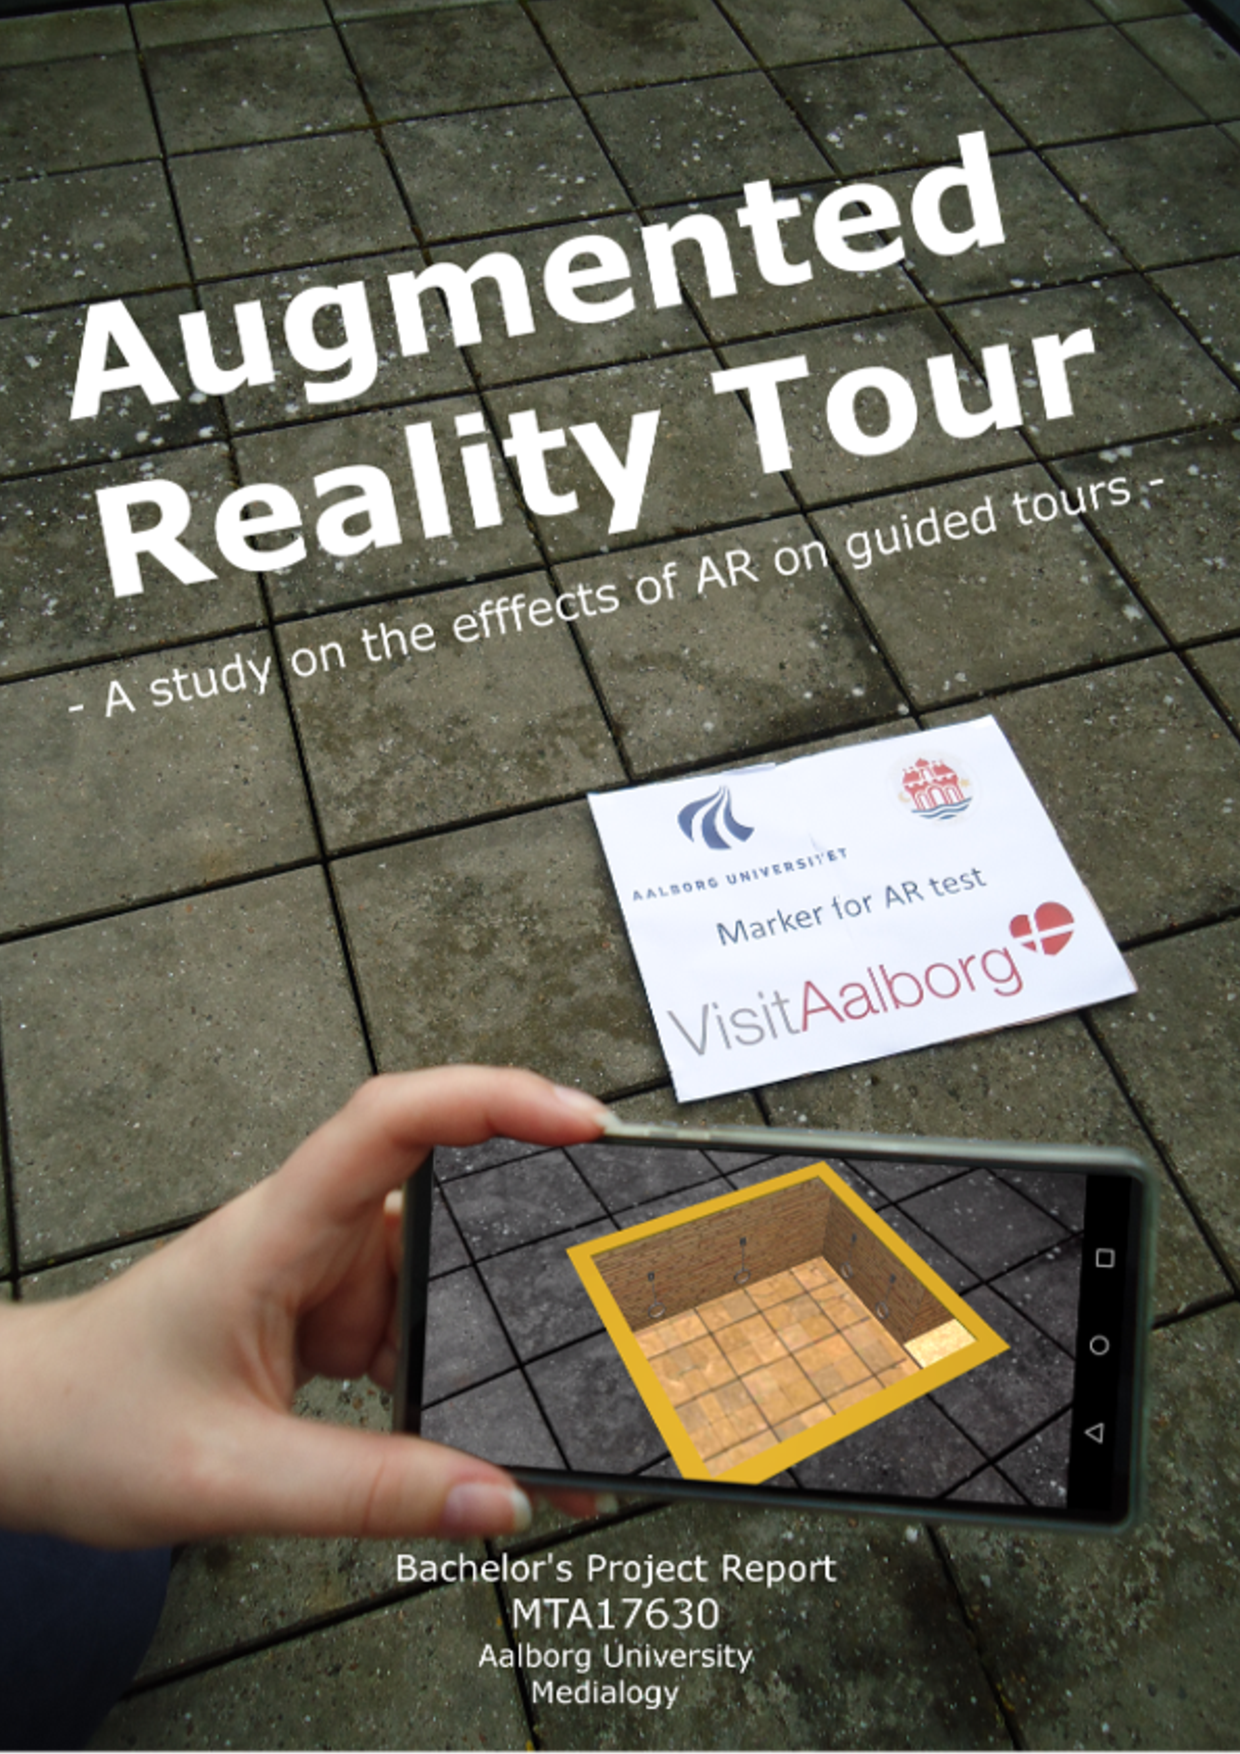
\includepdf{sections/frontpage_image.pdf}
\end{titlepage}
\clearpage


%\AddToShipoutPictureBG*{\includegraphics[width=\paperwidth,height=\paperheight]{figures/frontbg.jpg}};
\thispagestyle{empty}
{\small
\strut\vfill % push the content to the bottom of the page
\noindent Copyright \copyright{} Aalborg University 2015\par
\vspace{0.2cm}
\noindent Here you can write something about which tools and software you have used for typesetting the document, running simulations and creating figures. If you do not know what to write, either leave this page blank or have a look at the colophon in some of your books.
}
\clearpage


\pdfbookmark[0]{English title page}{label:titlepage_en}
\aautitlepage{%
  \englishprojectinfo{
    Augmented Reality Tour %title
  }{%
    Interactive Systems Design %theme
  }{%
    Spring Semester 2017 %project period
  }{%
    MTA17630 % project group
  }{%
    %list of group members
    Christina Kristensen\\ 
    Emilie Lind Damkjær\\
    Liv Arleth\\
    Margarita Kaljuvee
  }{%
    %list of supervisors
    Ivan Adriyanov Nikolov\\
    Claus Brøndgaard Madsen
  }{%
    1 % number of printed copies
  }{%
    \today % date of completion
  }%
}{%department and address
  \textbf{Medialogy}\\
  Aalborg University\\
  \href{http://www.aau.dk}{http://www.aau.dk}
}{% the abstract
\small{This is a research study into how augmented reality, when used to showcase a construction normally inaccessible to the audience, may impact the audience’s experience with a guided tour concerning curiosity invocation, entertainment value, and distraction level. An AR application was developed using Unity and Vuforia. The application shows a 3D model of a subterranean structure which becomes visible using the camera of a smartphone and a marker. To research this the method \textit{between design} was applied to a mock-up tour arranged in cooperation with a guide from Aalborg Guideforening. In accordance with this method, a control group would experience the tour through the guide’s normal narratives, and a test group would use the application in addition to the tour. By comparing results gathered from the two groups, a conclusion is drawn that the AR application does not obstruct the tour experience, and that it therefore has the potential to be integrated in an actual guided tour after further development and testing.}}
\cleardoublepage
\pdfbookmark[0]{Contents}{label:contents}
\pagestyle{fancy} %enable headers and footers again
\tableofcontents
\listoftodos
\chapter*{Authors\markboth{Authors}{Authors}}\label{ch:Authors}
\addcontentsline{toc}{chapter}{Preface}

\vspace{\baselineskip}\hfill Aalborg University, \today
\vfill\noindent
\\
\begin{minipage}[b]{0.45\textwidth}
 \centering
  Christina Kristensen\\
 {\footnotesize <ckris14@student.aau.dk>}
\end{minipage}
\hfill
\begin{minipage}[b]{0.45\textwidth}
 \centering
  Emilie Lind Damkjær\\
 {\footnotesize <edamkj14@student.aau.dk>}
\end{minipage}
\\
\\
\\
\begin{minipage}[b]{0.45\textwidth}
 \centering
  Liv Arleth\\
 {\footnotesize <larlet14@student.aau.dk>}
\end{minipage}
\hfill
\begin{minipage}[b]{0.45\textwidth}
 \centering
  Margarita Kaljuvee\\
 {\footnotesize <mkalju14@student.aau.dk>}
\end{minipage}
\\
\\
\\
\\
\\
\\
\cleardoublepage
%mainmatter
\pagenumbering{arabic} %use arabic page numbering in the mainmatter
\chapter*{Preface\markboth{Preface}{Preface}}\label{ch:preface}
This report documents the 6th semester Medialogy bachelor project committed in the period February to May 2017 by Christina Kristensen, Emilie Lind Damkjær, Liv Arleth, and Margarita Kaljuvee in connection to the semester theme \textit{Interactive Systems Design}.

For an optimal understanding, this report should be read in chronological order. In the end of the report miscellaneous appendices are alphabetically listed named by a capital letter from A-Z, which is used for the referencing in the report text. Listed in the bibliography, found last in the report, are references to previous work. The method used for the referencing here is the ACM SIGCHI method. This method has references alphabetically ordered based on the first author’s last name. To reference a text or an image, the report refers to the number given by this order.

As a supplement to the report, an AV production has been made. This summarises the scope of the project and its findings. Also to be found is a link to the application along with an electronic version of the marker including instructions to the usage of the developed system. All of this is gathered in the attached zip folder.

In closing, we in the group wish to dedicate our thanks to each person who has contributed to the outcome of this project. First of all we want to thank VisitAalborg and Aalborg Guideforening for their willingness to assist us. Especially a huge thank you to Inge Vestergaard, our contact guide, without whom this project would not have been possible. Secondly, we thank all the participants who volunteered to participate in our evaluation. Finally, we would like to express our gratitude to our supervisor Ivan A. Nikolov and co-supervisor Claus B. Madsen for their commitment and constructive advisory throughout the entire project.
\chapter{Problem statement}\label{ch:problemstatement}
Here goes the problem statement
\chapter{Background Research}\label{ch:backgroundresearch}
This chapter introduces the theories about augmented reality and human depth perception on which this project is based, as well as presents some reflections about the relation between the two. Lastly, a description of the state of the art provides some examples of existing systems with similar goals as those this project aims toward.

\section{Visual Depth Perception Within Humans}
Mathematical depth is to be thought of as the third dimension (first and second being length and width respectively). Depth is measured as the distance between two points in a vertical upward/downward and horizontal inward/outward direction depending on the objects of attention as well as angle of view (AOW) \cite{Gale}. Perception on the other hand defines the brain’s ability to sense and be aware of object’s existence through one or more of the five human senses: Hearing, smell, taste, touch, and vision. Of these the sense of vision --- primarily processed in the brain’s occipital lobe based on signals received from photoreceptors on the eyes’ retina registering the spatial, temporal, and chromatic components of light \cite{Spector2003} --- is considered the primary but not solemn sense for perceiving depth. As \textit{The Gale Encyclopedia of Science} states: \textit{“While depth perception results primarily from our sense of vision, our sense of hearing also plays a role.”} \cite{Gale}. Research with infants has further revealed that the ability to perceive depth visually within humans exist from as early on as two month of age \cite{Gale}. Thus it follows that visual depth perception within humans can be defined as the ability of humans with normal functioning eyes that follows the age of two month to use sight to see in three dimensions and estimate the spatial distances of objects from oneself and from each other.

\subsection{Depth cues}
For the brain to determine an object’s location in space and its relation to other objects certain estimates referred to as cues are used. Overall the cues can be separated into one of two types, namely monocular and binocular cues which are based on single eye and two eye information respectively. Furtheron, the monocular cue can be subdivided into pictorial cues and non-stereoscopic cues. To the pictorial cues belongs: Interposition, shading and lighting, aerial perspective, elevation, linear perspective, texture gradients, and retinal size, while the non-stereoscopic cues consist of motion parallax and accommodation. Meanwhile, members to the binocular cues are convergence and retinal disparity \cite{Gale}. 

\subsubsection{Monocular Depth Cues}
The following explains the aforementioned cues connected to monocular vision, meaning that these cues requires access to information from only one eye in order to be perceived.

\textit{Interposition} is when one object appears to be partially blocked by another object (as seen in Figure \ref{fig:cue0}), sometimes also referred to as occlusion or overlapping. During the image processing done by the brain this cue is used to determine which object should be perceived as the closest to the viewer since objects nearer the viewer tends to cover up parts of objects further behind \cite{Gale}.

\begin{figure}[h!]
   \centering
   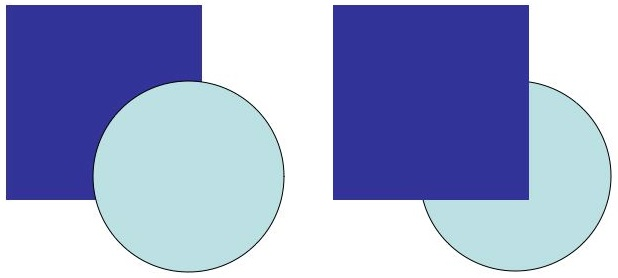
\includegraphics[width=0.7\textwidth]{figures/cue0.jpg}
   \caption{Interchange in occluded object to showcase the effect of interposition \cite{Heeger}}\label{fig:cue0}
\end{figure}

\textit{Shading and lighting} clues to the distance from the object to a light source as the surface closest to the light appears brighter than that of the surfaces further away which gradually darkens by the distance from the light source. Moreover, surfaces turned away from the light are perceived as dark progressing towards black the nearer they are to the light source. The viewer uses this to estimate whether to perceive the object as more convex or concave in shape \cite{Gale}. An example can be seen in Figure \ref{fig:cue1}.\pagebreak

\begin{figure}[h!]
   \centering
   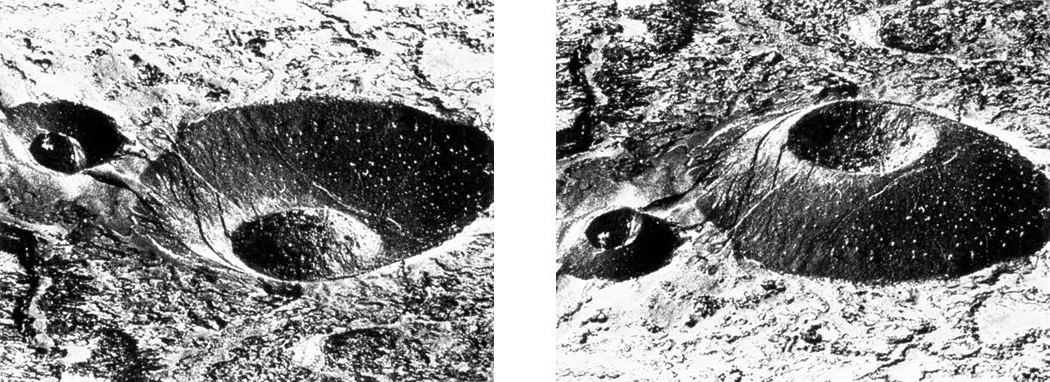
\includegraphics[width=\textwidth]{figures/cue1.jpg}
   \caption{Effects on the human depth perception by variations in shading and lighting \cite{Heeger}}\label{fig:cue1}
\end{figure}

\textit{Aerial perspective}, also known as \textit{atmospgeric perspective},  involves the sharpness of an object. From this it follows that the sharper an object is perceived by the eye, the nearer to the viewer the said object is interpreted to be, and the more blurred an object is perceived to be, the farther the distance seems between the object and the viewer. An example can be seen in Figure \ref{fig:cue2} The cause of this effect is the particles in the atmosphere e.g. water vapour and dust which either scatters or absorb light reflected by an object \cite{Gale}.  

\begin{figure}[h!]
   \centering
   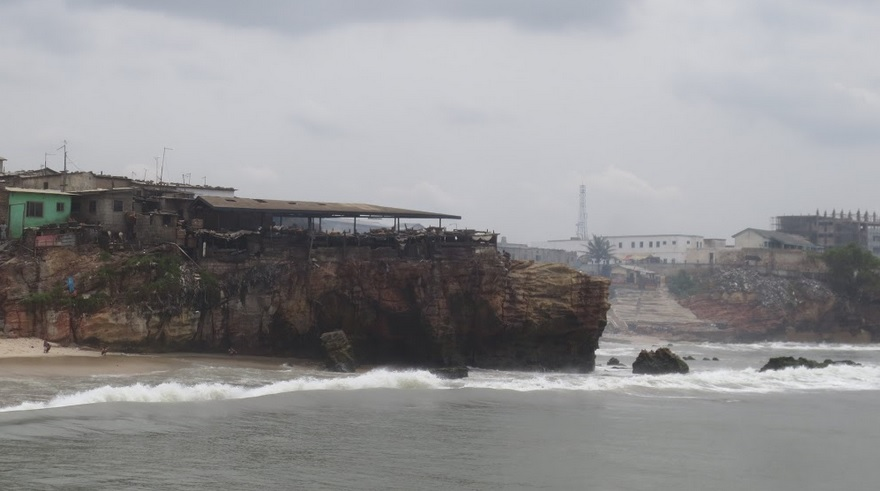
\includegraphics[width=\textwidth]{figures/cue2.jpg}
   \caption{Example of aerial perspective --- the buildings to the left are closer than the buildings to the right}\label{fig:cue2}
\end{figure}

\pagebreak
\textit{Elevation} considers the eyes’ placement of an object in correlation to the horizontal line, as can be seen in Figure \ref{fig:cue3}. Here the horizon (horizontal line, Figure \ref{fig:cue3}) is observed as either higher (foreground 1, Figure \ref{fig:cue3}) or lower  (foreground 2, Figure \ref{fig:cue3}) than that of the foreground. Thus objects placed near to the horizontal line is perceived as being in the distance in contrast to objects located near either the upper or lower outline of the visual field which are perceived to be nearer the viewer \cite{Gale}.   

\begin{figure}[h!]
   \centering
   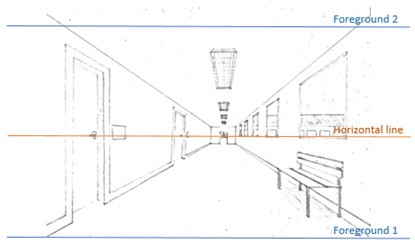
\includegraphics[scale=0.8]{figures/cue3.jpg}
   \caption{An example of elevation}\label{fig:cue3}
\end{figure}

\textit{Linear perspective} is the correlation occurring between the decrease in an object’s size and separating spaces on the retina when repeatedly lined up along a line and the perceived increase in distance from the point of view (POW) until the vanishing point is reached where the object cease to be visible, as can be seen in Figure \ref{fig:cue4} \cite{Gale}.

\begin{figure}[h!]
   \centering
   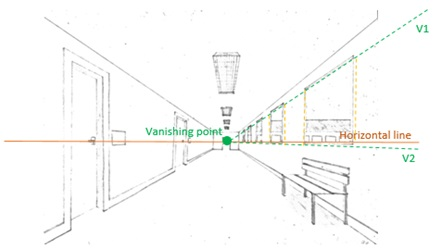
\includegraphics[scale=0.8]{figures/cue4.jpg}
   \caption{An example of linear perspective}\label{fig:cue4}
\end{figure}

\textit{Texture gradients} concerns the affection of texture perception by an increase in distance whereto it follows that by increased distance the size of elements that make up the surface texture appear to be smaller while the distance between said elements seems to decrease, as seen in Figure \ref{fig:cue5} \cite{Gale}.

\begin{figure}[h!]
   \centering
   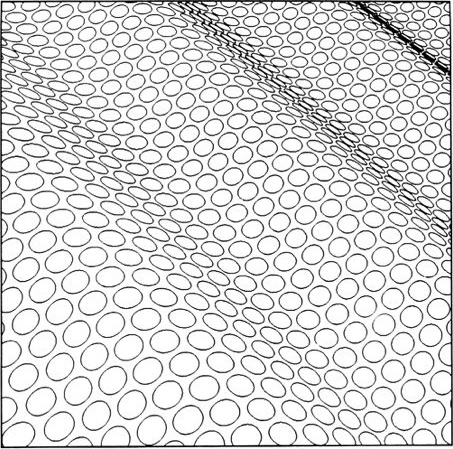
\includegraphics[width=0.4\textwidth]{figures/cue5.jpg}
   \caption{Texture gradient \cite{Heeger}}\label{fig:cue5}
\end{figure}

\textit{Retinal size} considers the brains automatically distinguish between an object being distant or near, interpreted based on the retinal image recognition of an object as small or large respectively, utilised in case of the absence of additionally visible cues to suggest the opposite. Thus, as it can be seen in Figure \ref{fig:cue6} the dotted arrow A, although having the same size as the arrow B, looks larger when comparing the projections of A and B on the retina, and hence it is considered to be nearer. However, as it is to be seen from the two airplanes in Figure \ref{fig:cue7} this method for distinguishing distance only applies for objects of the same size since a larger object located farther away may look the same size on the retina if compared to a nearer small object \cite{Gale}.

\begin{figure}[h!]
   \centering
   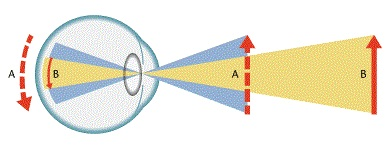
\includegraphics[scale=0.7]{figures/cue6.jpg}
   \caption{Retinal size used to infer distance \cite{Perslides}}\label{fig:cue6}
\end{figure}

\begin{figure}[h!]
   \centering
   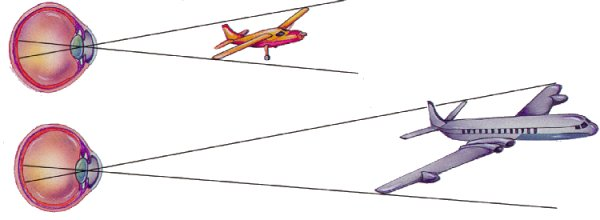
\includegraphics[scale=1]{figures/cue7.jpg}
   \caption{Retinal size, wrong interpretation of reality \cite{Psych}}\label{fig:cue7}
\end{figure}

\pagebreak
\textit{Motion Parallax} is the perception of apparent motion of two stationary objects with relative different distances to the viewer (located respectively in front of and behind of the viewer’s fixation point) caused by changes in the viewer’s position. This reasons in the movement of the eyes in relation to the spatial environment, because whenever a person move, the images projected by objects located at different distances as a result of said movement comes to move across the retina with different speed. To this it can be said that objects relative close to the viewer is perceived as moving at a higher speed when compared to objects located in the distance. Further on will the near object seem to be moving in the opposite direction as the viewer whereas the farther away object will be heading in the same direction as the viewer.  In addition to this it is also noticeable that distant objects seem to move smaller distances than that of objects near the viewer \cite{Gale} \cite{Shrestha2013} \cite{Skybrary}.

\begin{figure}
	\centering
	\begin{subfigure}[h!]{0.4\textwidth}
		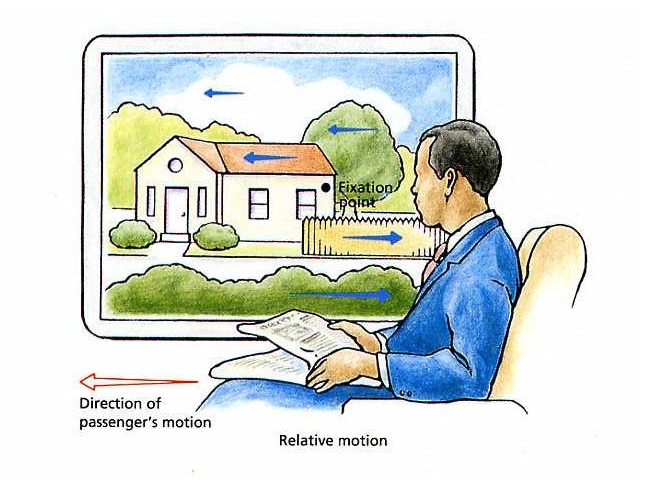
\includegraphics[width=\textwidth]{figures/cue8.jpg}
		\caption{Experiencing motion parallax \cite{Parallax0}}\label{fig:cue8}
	\end{subfigure}
	\begin{subfigure}[h!]{0.4\textwidth}
		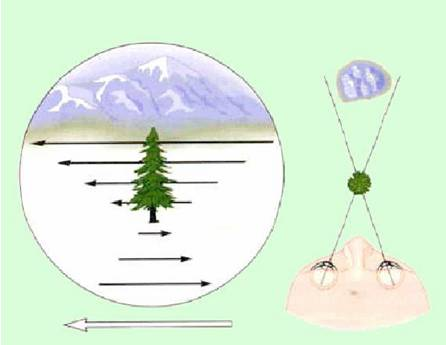
\includegraphics[width=\textwidth]{figures/cue9.jpg}
		\caption{Motion parallax explained \cite{Skybrary}}\label{fig:cue9}
	\end{subfigure}
	\caption{Illustrations demonstrating motion parallax}
\end{figure}

\begin{figure}[h!]
   \centering
   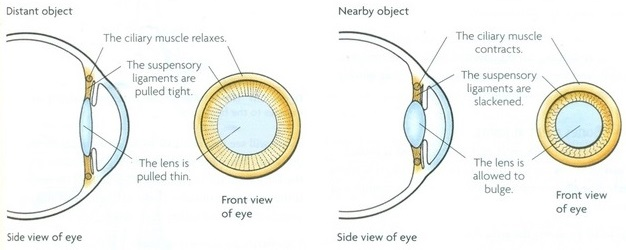
\includegraphics[width=0.8\textwidth]{figures/cue10.jpg}
   \caption{Accommodation, left: Distant focused lens, right: Near focused lens \cite{Biology2014}}\label{fig:cue10}
\end{figure}

\textit{Accommodation} is the physiological changes happening to the lens’ curvature to sharpen the retinal images of near and far objects. In order to have the eye focus on a distant object the lens have to flatten (Figure \ref{fig:cue10}, left). Meanwhile, to focus on near objects the lens becomes more of a curve (Figure \ref{fig:cue10}, right). These changes in the lens’ curvature are controlled by the ciliary muscle which seemingly sends signals as feedback to the brain about alterations in the muscle tension that may assist in determining the distance to the object \cite{Gale}.

In addition to monocular cues comes the semi-cue: Familiarity which is used in other sections of human’s visual processing as well. This takes as its starting point an individual’s previous experience with the spatial characteristics of various objects and contributes to determine the distance to the object thereby assisting in the spatial perception \cite{Gale}

\subsubsection{Binocular Depth Cues}
This will describe the two cues connected to binocular vision which means that the cues requires access to information from both eyes in order to be perceived.

\textit{Convergence} takes into consideration the eyes’ propensity to rotate inward toward each other in a coordinated manner in furtherance of an effectively focus on objects close to the eyes. In opposition to this the focus on distant objects have the eyes move outward toward the temples. However, changes in convergence cease to befall when an object exceeds the approximately distance of six metres from the eyes. Here the eye pupils reaches a point where they are essentially parallel to each other and cannot move any further away. It seems that the resulting muscular tension changes in the eye muscles that are required to cause these convergent eye movements in order to focus on near and far objects provide feedback to the brain about the depth or distance \cite{Gale}.

\begin{figure}[h!]
   \centering
   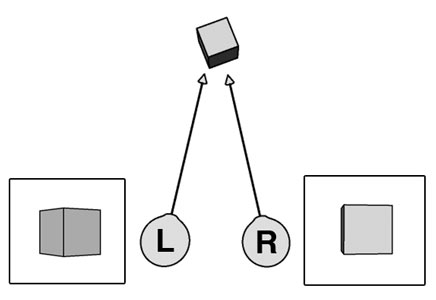
\includegraphics[width=0.4\textwidth]{figures/cue11.jpg}
   \caption{Example of retinal disparity between  left and right eye \cite{Retina}}\label{fig:cue11}
\end{figure}

\begin{figure}[h!]
   \centering
   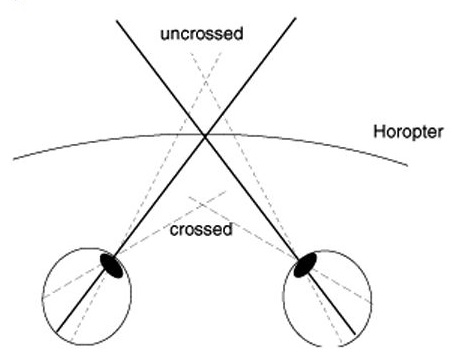
\includegraphics[width=0.4\textwidth]{figures/cue12.jpg}
   \caption{Distinction between crossed and uncrossed disparity \cite{Heeger}}\label{fig:cue12}
\end{figure}

\textit{Retinal disparity} is caused as a result of humans’ laterally arrangement of the two eyes which provides a positional difference (an interocular distance of 60 to 65 mm). This positional difference let us see the world from two slightly different points of perspective. Disparity here occurs where a singled out object in the images constructed in each of the two eyes do not stimulate corresponding points on the respective retinae hereof the name: ‘retinal disparity’ (or binocular disparity).  Mainly these differences happens in the relative horizontal position of objects which is why they are also sometimes referred to as horizontal disparity, and is defined by McCoun and Reeves as: \textit{“the difference in position of corresponding points between images in two eyes”} \cite{McCoun2010}.

Set into relation to the convergence of the eyes when focused on a fixed point (FP), retinal disparity can moreover be classified as either crossed or uncrossed. From FP an imaginary 3D surface called the horopter can be made consisting of all the positions in the two retinae that correspond (Figure \ref{fig:cue12}). If a point is perceived as within the range closer than that of FP it in general has lines of sight that cross in front of the horoptor. Such an occurrence is called a crossed disparity (Figure \ref{fig:cue12}). Alternatively do any point positioned beyond the range of FP typically have lines of sight meet behind the horoptor, resulting in the lines not crossing each other before this point, hence the name uncrossed disparity (Figure \ref{fig:cue12}) \cite{McCoun2010}.

When the subtle differences between the retinal images from the eyes are forwarded to the brain neural processes merge them such that they become a single percept. This produces a series of smaller disparities that permits a specific form of depth perception known as stereopsis, and its perceived visual result is a 3D image \cite{Parker2007}.

\subsection{Reflections Upon Human Depth Perception in The Context of AR}
A major part of an AR system is to have the digital 2D overlay image appear as an integrated part of the real world environment generated by the real time video transmission, and since any camera imitates the eye’s retina in the way it produces its images. Thus it befalls that the retina based cues for depth perception in the human eye also applies to a camera’s way of processing the sense of depth in an image.

\begin{figure}[h!]
   \centering
   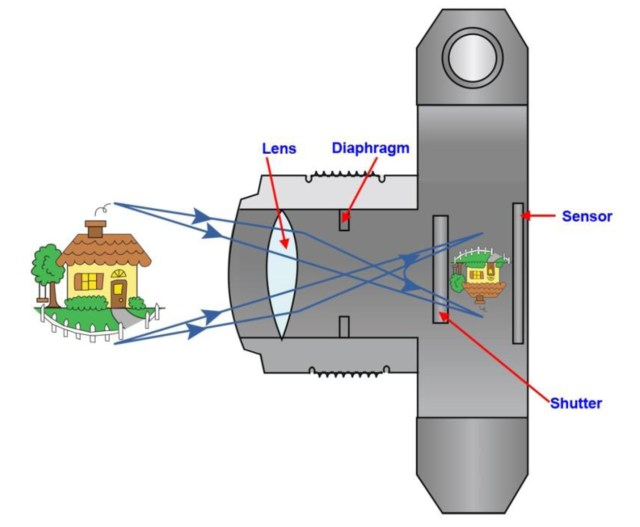
\includegraphics[width=0.5\textwidth]{figures/camera.jpg}
   \caption{Camera image production \cite{Camera}}\label{fig:camera}
\end{figure}

To this it has to be added that unless two cameras are used to produce the image, one only have to consider the monocular depth cues, given that the binocular cues requires two eyes, or in this case two cameras, in order to be obtained. This further means that the pictorial depth cues becomes the primary source for integrating a digital AR overlay into a real time footage, because the non stereoscopic monocular depth cues relates to physical movement or changes in the eye muscles for which reason they are outside the AR system’s control.

\section{Augmented Reality}
As suggested by Madden in the book Professional Augmented Reality Browsers for Smartphones, AR is to be thought of as the opposite of Virtual Reality (VR). As Madden explains it: “Virtual reality immerses the user in a computer-generated world whereas AR combines the real world with computer graphics.” \cite{Madden2011}. Moreover, Madden points out that where it requires the user to acquire special equipment to experience VR, AR requires only a device able to capture the environment (e.g. a smartphone or tablet) as well as methods to experience the computer world typically in the form of an overlaying computer graphic in the camera window \cite{Madden2011}. Based on this, Madden defines AR as a technology which combines the real world with computer graphics, tracking and/or providing interaction with objects in real-time. Furthermore, AR provides recognition of images or objects, as well as delivering real-time context or data. By utilising this definition Madden allows technologies to be included that are not considered AR in the strictest interpretations e.g. AR browsers \cite{Madden2011}.

In relation to the above definition of AR, Madden makes a distinction between two tracking systems, namely tracking by markers and markerless tracking. The method of tracking by markers makes use of patterned images, which activate a certain action when recognised. Examples of markers are the fiduciary marker, Quick response codes (QR), and Microsoft Tags. Markerless tracking on the other hand works by tracking objects in the real world not using markers made for the purpose. An example of markerless tracking is facial recognition \cite{Madden2011}.

Approaches to mobile AR are mainly split into two paths, namely AR using location and orientation data to compute what is viewed, and AR using actual image content captured by a camera to compute what is viewed referred to as \textit{computer vision}.

As introduced by Madsen and Lal, Aalborg University, in the book Augmented Reality, chapter 2 \cite{Lal2010}, AR can be associated with three major challenges:

\begin{enumerate}
\item Camera tracking 
\item Handling occlusions
\item Illumination consistency
\end{enumerate}

The obstacle with camera tracking involves \textit{“matching position and orientation of the camera to the coordinate system of the scene”} \cite{Lal2010}, which deals with making sure the angle of the scene captured by the camera matches that of the virtual scene. Handling occlusions means \textit{“having sufficient 3D information of the real scene to handle occlusion between real and virtual geometry”} \cite{Lal2010}, so that real-world objects such as people walking by may occlude the virtual objects. Lastly, illumination consistency deals with the problems of \textit{“having sufficient knowledge of the real scene illumination to be able to render virtual objects with scene consistent illumination, including shadows”} \cite{Lal2010}. The latter of these three is especially important for creating visually credible AR in outdoor environments because of this scenario’s dynamically changing illumination.

\section{State of the Art}
Augmented reality can be used to various ends. The popular game Pokémon Go, which was released in the summer of 2016, includes an optional AR feature \cite{Pokemon}. However, AR has also been utilised for tourism. Feiner et al. (1997) developed a system which allowed users to access access information about a campus using an overlay interface \cite{Feiner1997}. Because of the age of this prototype, however, a bulky setup was required, including a backpack-worn computer and a head-mounted display. A prototype built by Fritz et al. (2005) uses a camera, binoculars and internal sensors to augment a video stream with graphical objects, such as information of a site, or visualisations of what a site looked like in the past \cite{Fritz2005}. A sketch of this prototype is seen in Figure \ref{fig:binoculars}.

\begin{figure}[h!]
    \centering
    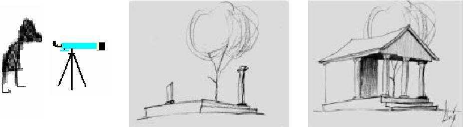
\includegraphics[scale=0.7]{figures/binoc.png}
    \caption{Sketch of Fritz et al.'s prototype (left), the unaugmented image (middle), and the augmented image (right) \cite{Fritz2005}}\label{fig:binoculars}
\end{figure}

While a majority of AR solutions for tourists are scientific prototypes, a few commercial products are available for mobile smartphones. Using apps such as Wikitude, users can experience several different types of AR experiences, as developers are able to upload their AR project to the platform. This allows various third-party stakeholders to utilise the app. A screenshot of Tripadvisor's use of the Wikitude platform can be seen in Figure \ref{fig:wikitude}. The app uses different input methods to load the AR experiences, such as GPS location, images, and QR-codes \cite{Wikitude}. It primarily functions as a platform for AR advertisements or similar commercial products.

\begin{figure}[h!]
    \centering
    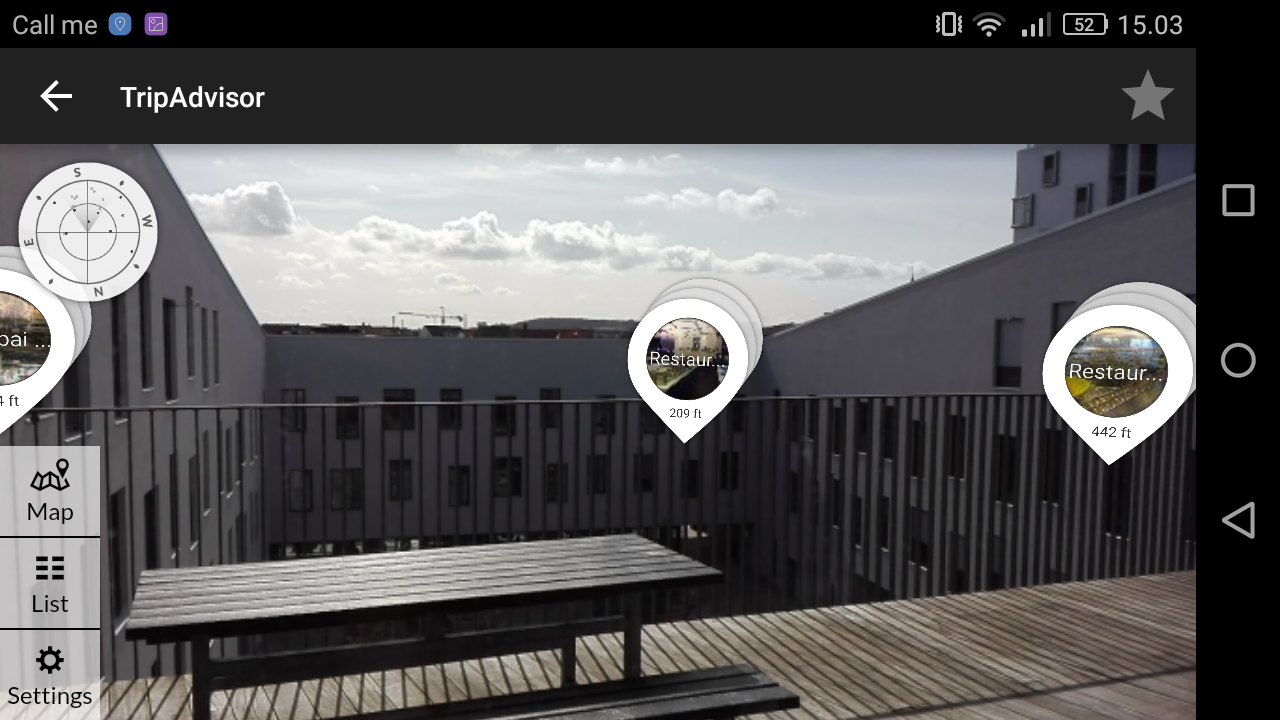
\includegraphics[width=0.65\textwidth]{figures/wikitude.png}
    \caption{Screenshot of the Wikitude app, as utilised by Tripadvisor}\label{fig:wikitude}
\end{figure}

The Yelp app, dedicated to reading and writing reviews of local restaurants, has an optional feature called \textit{monocle}, which allows users to see the average rating of nearby restaurants based on location \cite{Yelp}. A downside to this feature is that depending on the density of nearby restaurants, the screen may get quite cluttered, as can be seen in Figure \ref{fig:yelp}.

\begin{figure}[h!]
    \centering
    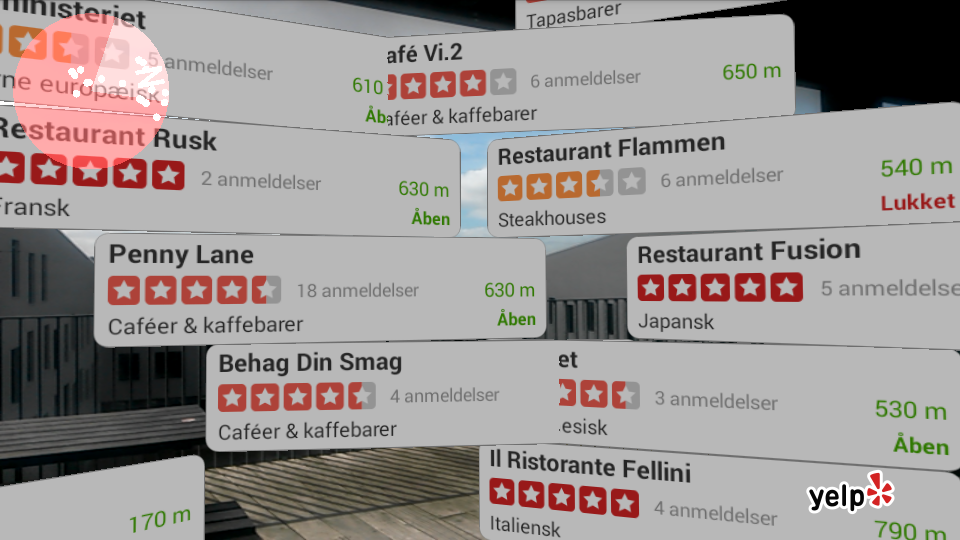
\includegraphics[width=0.65\textwidth]{figures/yelp.png}
    \caption{Screenshot of the Yelp monocle feature}\label{fig:yelp}
\end{figure}

%I am just commenting this out in case we need it
%Here is equation~\eqref{eq:esun}:

%\begin{equation}
%\label{eq:esun}
%E_{sun} = (\vec{n} \cdot \vec{s}) \times \_E_{sun}
%\end{equation}
\chapter{Design and Implementation}\label{ch:implementation}
Implementation goes here.\todo{write an intro here}

\section{Preliminary Interest Test}
For the purpose of testing different methods of data gathering for the evaluation a preliminary test was conducted. This test also served the purpose of obtaining a baseline for the length of time users might spend on an AR application, which also served as an answer to research question 1.

\subsection{Metrics}\label{subsec:premetrics}
For this test four different sets of data were gathered. Two of the metrics were self-reporting, meaning the participant chose the answer. The other two metrics were data gathered by the sensors attached to the arduino and to the participant. The four parameters are as follows:
\paragraph{Electrodermal activity (EDA):} The EDA sensors measure the skin conductance of the wearer. This is used to read the wearer’s level of arousal, which rise and fall depending on the task of the wearer and how exciting they find the task. The more aroused the wearer is, the more sweat will be generated and thereby increasing the conductance.
\paragraph{Inter-Beat interval (IBI):} The IBI sensor measures the heart rate variability (HRV) which varies from beat to beat, by recording the beats of the pulse. The more relaxed a person is the more variability there is between the beats, and vice versa. 
\paragraph{Time:} Throughout the experiment, the time is recorded so that other parameters may be compared to it. This was done by having the facilitator stop the timer when receiving a notice from the participant to stop, since the equipment work by the participant during the test prohibited them from stopping the timer themselves.
\paragraph{Self-assessment manikin (SAM):} As described by Bradley and Lang (1994), the \textit{self-assessment manikin} (SAM) is a picture-oriented instrument to assess a subject’s pleasure, arousal, and feeling of control in response to a stimulant. The three rows, seen in Figure \ref{fig:SAM}, each represent one of these parameters on a 5-point scale with graphic depictions \cite{Bradley1994}. Subjects may point at the image which best represents their feeling of pleasure, arousal, and control.

\begin{figure}[h!]
    \centering
    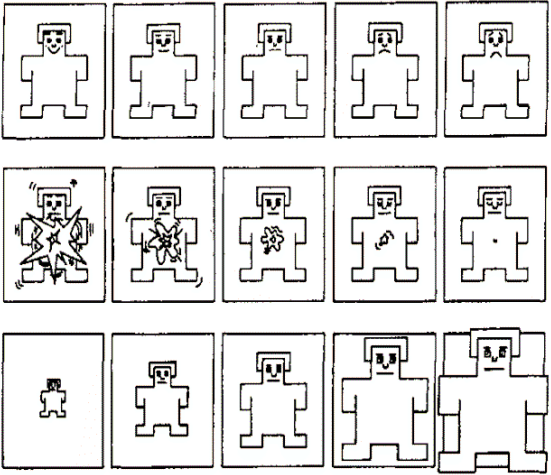
\includegraphics[width=\textwidth]{figures/SAM.png}
    \caption{The three SAM scales: Pleasure (top), arousal (middle), and control (bottom) \cite{Bradley1994}}\label{fig:SAM}
\end{figure}

\pagebreak

\subsection{Setup}
The following tools are used for the purposes of the preliminary interest test:

\begin{itemize}
    \item A smartphone with the AR app \textit{AR Dino Roar} installed
    \item An arduino with breadboard (as well as the necessary wires to connect everything)
    \item Two EDA sensors
    \item A pulse sensor
    \item A smartphone to serve as a stopwatch
    \item A computer to which the arduino is connected
    \item A camera to film the procedure
    \item A piece of paper with a pattern to serve as an AR marker
    \item A piece of paper showing the SAM scales
\end{itemize}

\textit{AR Dino Roar} is an application for android devices in which users may use their own pattern as an AR marker. The app then displays a model of a dinosaur in AR. A screenshot of this app can be seen in Figure \ref{fig:dino}.

\begin{figure}[h!]
	\centering
    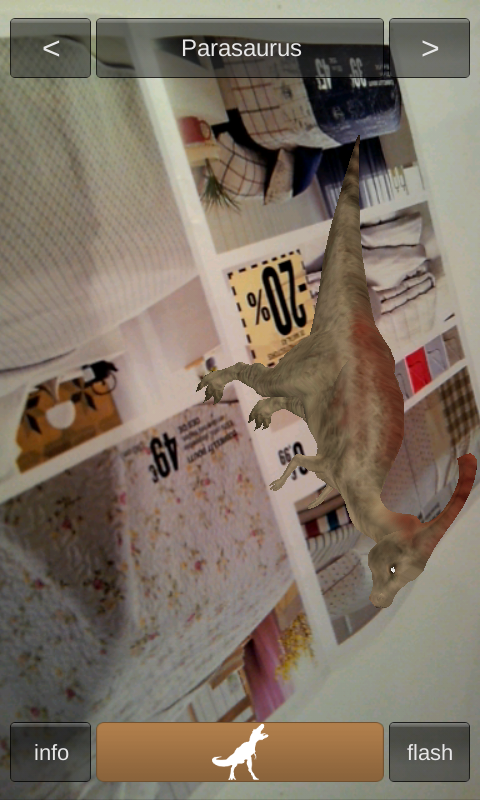
\includegraphics[scale=0.5]{figures/AR_dino.png}
    \caption{A screenshot of the AR Dino Roar app \cite{ARDino}}\label{fig:dino}
\end{figure}

In the test setup, a circuit is set up with the arduino, breadboard, sensors and wires in such a way that one can measure a participant’s EDA and IBI. The arduino is connected to the computer so that this data may be recorded. The EDA sensors are attached to the left index and middle finger of the participant, and the pulse sensor is attached to their left ear lobe, as seen in Figure \ref{fig:pretest_ear}.

\begin{figure}[h!]
    \centering
    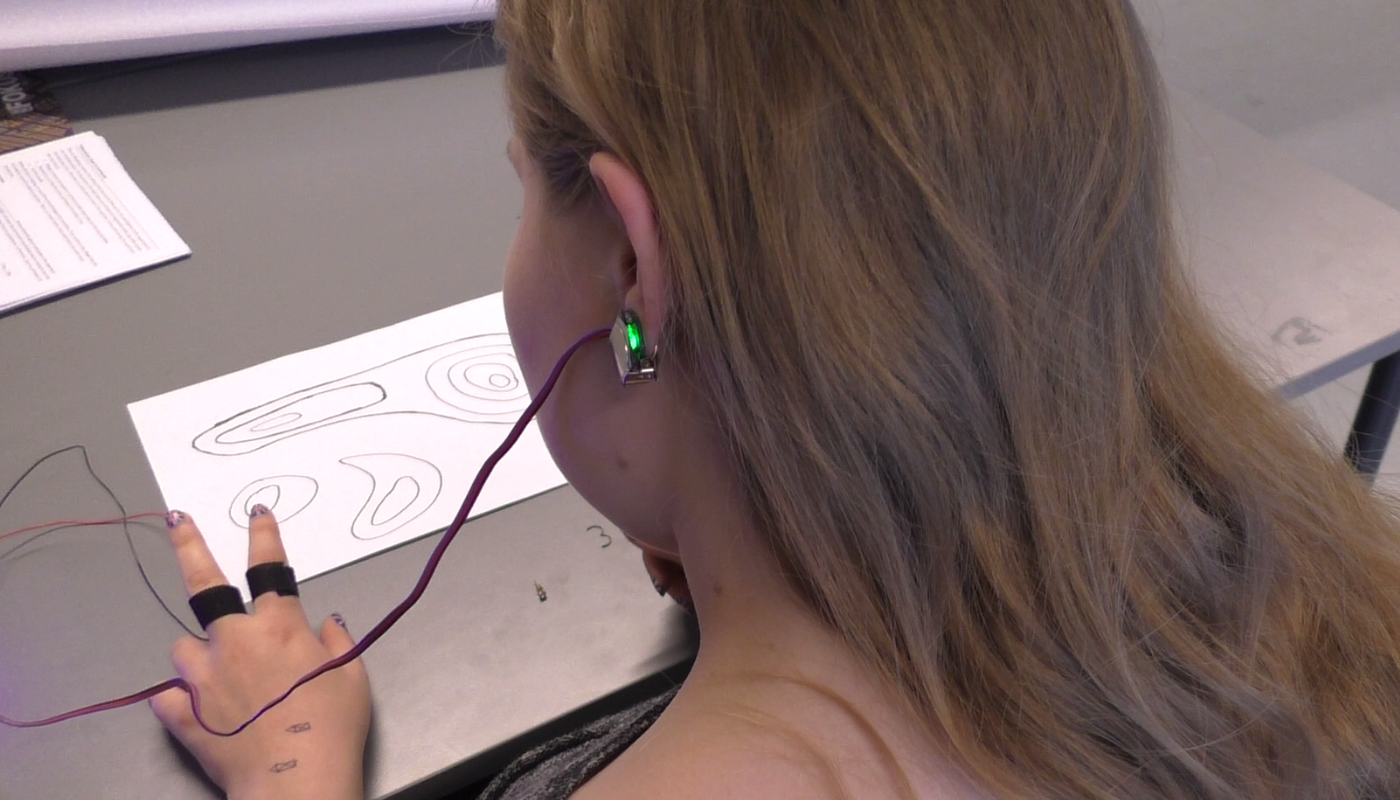
\includegraphics[width=0.8\textwidth]{figures/pretest_ear.png}
    \caption{The EDA and pulse sensors attached to a participant}\label{fig:pretest_ear}
\end{figure}

The test participant is seated in front of a table. On this table is the AR marker, the two smartphones, the SAM paper, and the arduino to which the participant is connected. The test facilitator is seated next to the participant in front of a computer, on which they record results from the test. The full test setup can be seen in Figure \ref{fig:pretest_setup}.

\begin{figure}[h!]
    \centering
    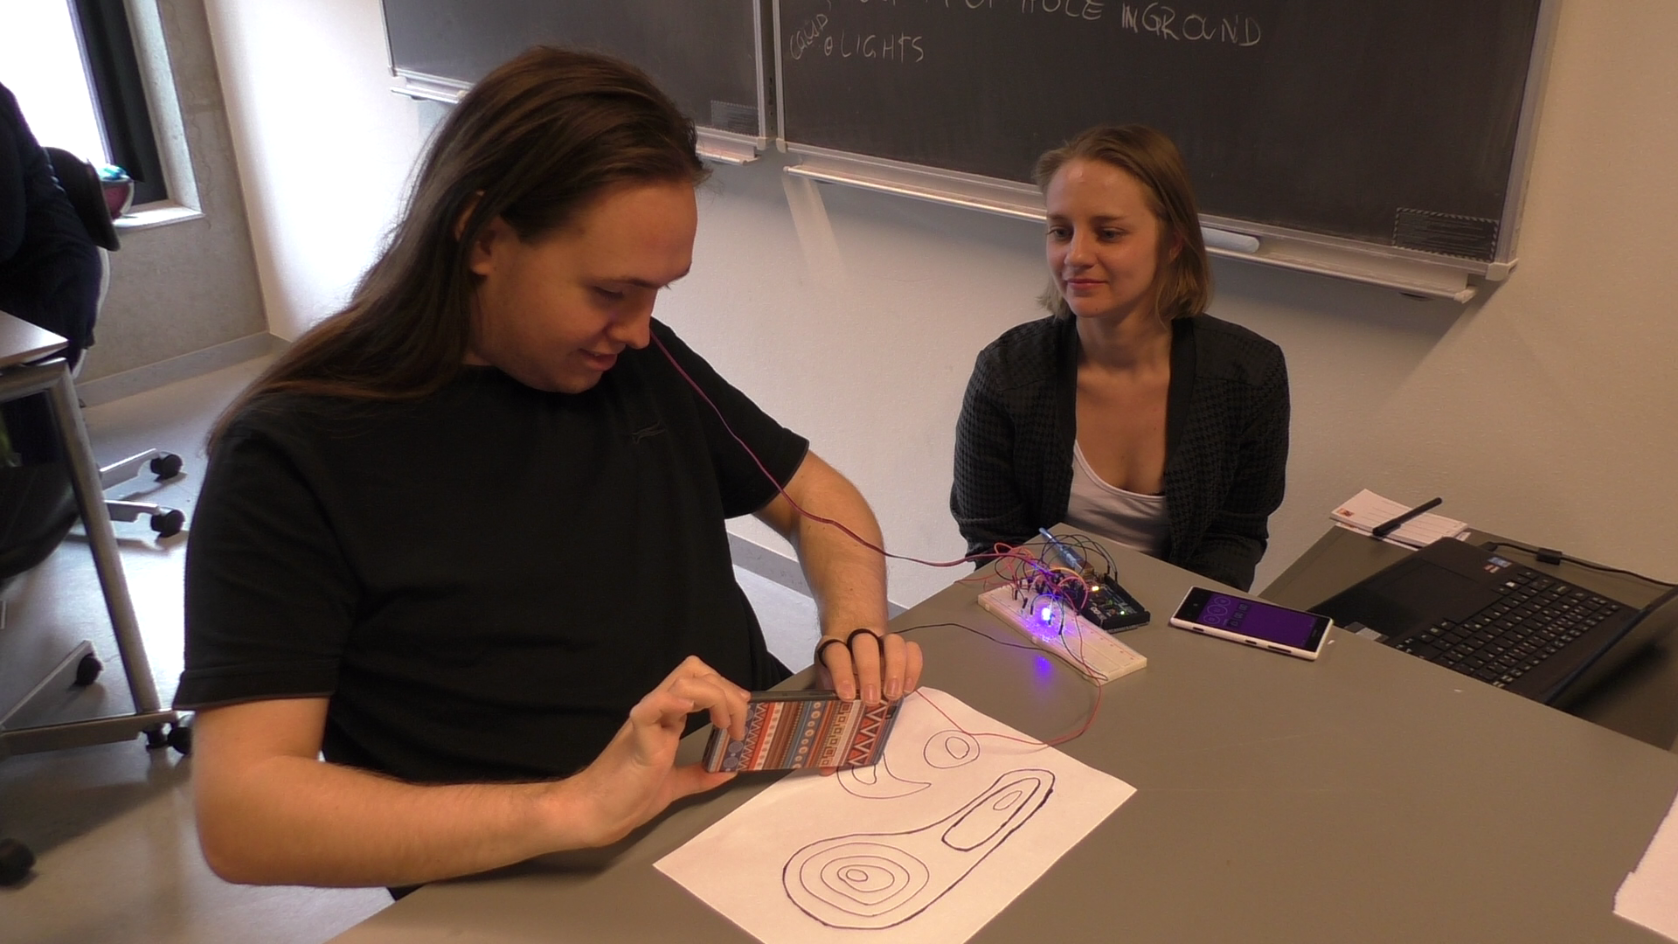
\includegraphics[width=0.8\textwidth]{figures/pretest_setup.png}
    \caption{The setup for the preliminary interest test}\label{fig:pretest_setup}
\end{figure}

\subsection{Procedure}
Before the test begins, the facilitator explains the procedure to the participant. They then attach the sensors to the participant as described in the previous section. Before the participant interacts with anything, they must sit idly for one minute, so that a baseline IBI and EDA may be recorded. They are then asked to use the AR Dino Roar app to look at a virtual dinosaur. The stopwatch is started once they begin, and they are asked to tell the facilitator to stop the timer once they are no longer interested in the app. Their IBI and EDA is recorded while they interact with the app. Once they are done interacting with the app, they are asked to answer three questions using the SAM diagram: how pleased, aroused, and in control they felt, respectively. For each question, they were asked to point to one of five images in a given row which best described their feelings, as described in section \ref{subsec:premetrics}.

\subsection{Analysis of results}
Out of the ten tests only seven sets of data were usable in regards to the logging of the sensor data. At some point after test number 5, something happened to make the data unstable and faulty. It is likely that loose wires are at fault. This means that only seven sets of data from the EDA and IBI sensors are useful, which is not enough to make a clear conclusion on arousal or HRV. The graphs, seen in appendix \ref{ch:appA}, are all very stable.

The average time participants spent on the app is 52.20 seconds. However, the data gathered from the timer comes with two outliers caused by unintended interaction with the app and technical issues respectively. These outliers have a considerably impact on the average time, which when leaving out the outliers comes down to 37.75 seconds. 

The pictures in each row of the SAM sheet are labeled 1 through five, so that 1 corresponds to most pleased, most aroused, and least in control, and 5 corresponds to least pleased, least aroused, and most in control. This makes it possible to find the median of each scale. The median response for level of pleasure is 2, which is the slightly pleased manikin. The median response for arousal is 4, which is the second-least aroused manikin. The median response for control is 2.5, meaning that the median falls between the second-least in control and the neutral manikin. It is possible that the low level of arousal and control is caused by the low level of interactivity to the app, as there is little to do but look at a static AR projection of a dinosaur. Despite the low ratings of these aspects, test participants felt slightly more pleasure than neutral. 

\subsection{Discussion}
The primary purpose of this test was to learn how long a user will spend on an AR application with no features other than showing a model. The test only had 10 participants, which is not an adequate number to base a conclusion on, but it is adequate to describe a tendency or to establish a baseline for further testing. Out of the four different metrics measured, only two were useful for this purpose because of the faulty data. 

One was measuring the amount of time they used the app until they stated that they were no longer interested. The average for this test was 52.20 seconds, however removing two outliers reduced it to an average of 37.75 seconds. This can be used as a baseline for how long we expect the participants to use the app during the evaluation.

Additionally, the SAM gave useful information. The parameters allow users to articulate through images how their experience was. A similar inquiry may be made in the final evaluation of this project. A factor to consider with all three SAM scales is the context of usage. For this test, the participants had no outside context to use the application (such as a tour guide explaining material which is relevant to what can be seen on the screen), and this might have affected the overall experience. 

The EDA and IBI data was very inconclusive, and due to technical difficulties only a bit more than half of the data was valid. This means that it would be inappropriate to use it for the final evaluation, especially since it would also be cumbersome and resource-heavy to bring it for the evaluation which will not be stationary and moreover takes place outside with several participants at a time.

\section{Minimum Implementation Requirements}
To define the minimum implementation requirements by priority the MoSCoW method developed by Dai Clegg \todo{\cite{Kuhn}} is used to sort the various features for the concept. MoSCow in itself is an acronym which is derived from the first letter of each priority category (Must have, Should have, Could have, and Won’t have but would like). Listed the MoSCoW priorities read as follows:

\textbf{Must have}:
\begin{itemize}
\item A 3D model placed such that it seems to be a hole in the ground when projected onto an image of the street
\item Ability to read a marker and project a 3D model onto it
\end{itemize}

\textbf{Should have}:
\begin{itemize}
\item Shaders and textures for the 3D model to make it look like a dungeon
\item Appropriate light setting
\item Details to the model such as a staircase and chains
\item The model should be angled in such a way that its perspective lines up with the images captured by the camera
\end{itemize}

\textbf{Could have}:
\begin{itemize}
\item Additional details to the model, such as a prisoner, straw, dirt etc.
\item Realistic looking light based on predictable information
\end{itemize}

\textbf{Won’t have but would like}:
\begin{itemize}
\item Markerless detecting system
\item Light adjustment system that adapts to weather type and time of day
\end{itemize}

It is found to be of the utmost importance to have a basic 3D model of the subterranean site. Further it is paramount for the users to be able to project this model onto their smartphone screen by registering a marker of some sort. The reasoning behind this priority is that the project first and foremost is about showcasing non-visible scenes occurring on a guided tour and see if this impacts the user experience, cf. the problem statement. 

It has also been deemed to be of some importance to have the model equipped with appropriate shaders and textures lit by a proper set of light sources. As it is explained in the previous chapter, a research study found that textures and shading in accordance with the light improves the 3D percept. Alongside, the texture in relation to the light choices should emphasise the atmosphere of a dungeon. Therefore some explanatory additions to detail the purpose and context of the model should be added e.g. stairs to state it to be on the lowest level (basement level), and chains to indicate prison. 

Of less importance is considerations to a realistic light setting in accordance with the predictable environmentals (e.g. existing buildings and sun orientation at a specific time of day) as well as higher levels of details to the model. Although details like piles of straw, dirt, prisoners, etc. could potentially improve the emphasis to the model and its contents, it is not part of the project’s main objective. Also despite having a light adjusting system which adapts to different weather conditions and time of day would be a nice addition which could add on to the realism of the scene, this has been considered out of the project scope. Lastly, though a markerless system would be a practical part of the finished application since this would make it easier for the guide to manage the application compared to bringing markers along, for the test purpose such a system has been found unnecessary to implement.


\section{Implementation}
To create an AR application, the plugin Vuforia was used in combination with Unity. The 3D models were created in Autodesk Maya 2015. The implementation process is described in further detail in the following sections.

\subsection{From Sketch to Model}
\begin{wrapfigure}{r}{0.35\textwidth}
\centering
        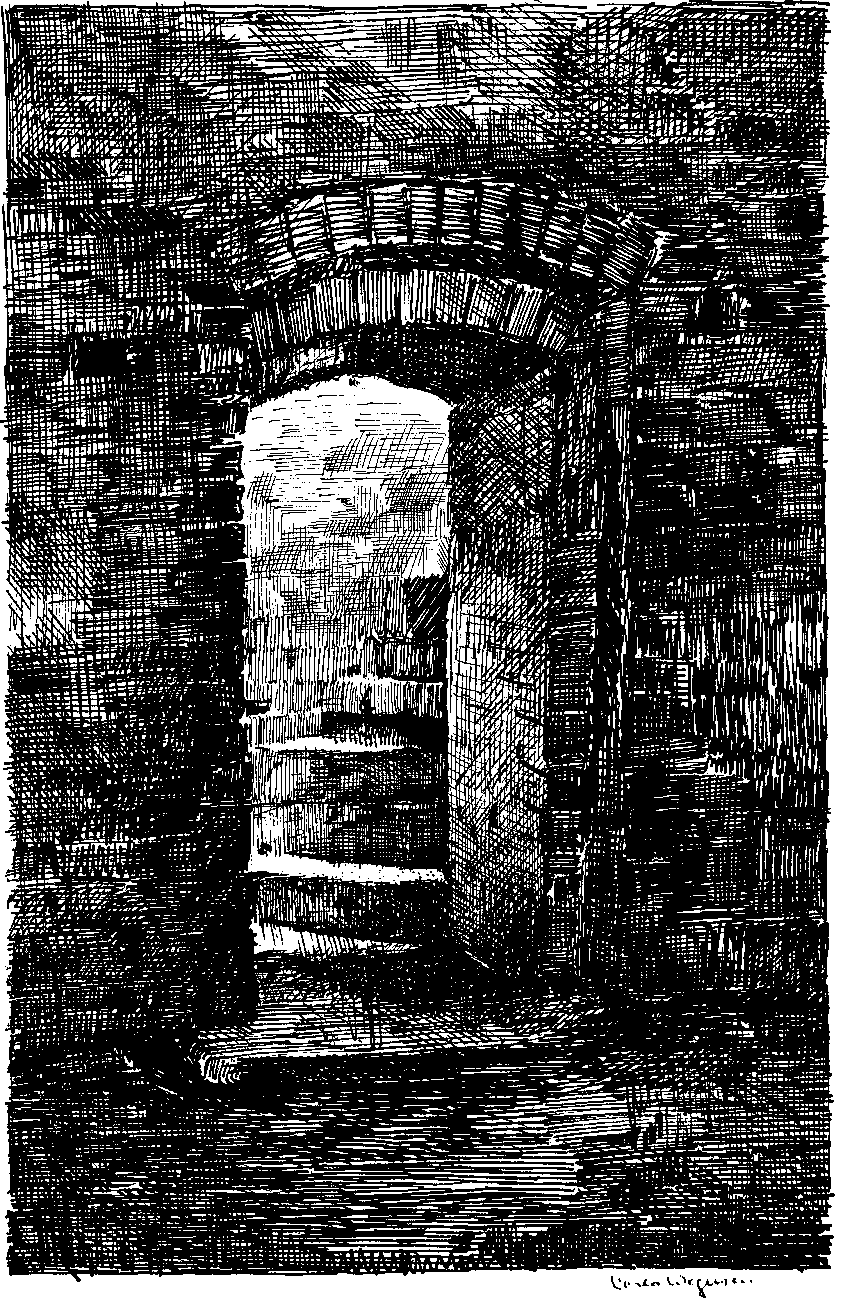
\includegraphics[width=0.3\textwidth]{figures/sketch1.png}
        \caption{Illustration by Carlo Wognsen of the dungeon beneath Vesterport, south wall with access to spiral staircase leading up to street level \cite{Riismoller1961}}\label{fig:sketch1}
\end{wrapfigure}

In order for the 3D model to be representative to the real “Rakkerens Hule”, the dimensioning and shape is primarily inspired by the architectonic sketches made of the excavated ruins of the prison at the western city gate of old Aalborg after its rediscovery in 1907. These were prepared by architect H. Paludan at the request of Nationalmuseet, see Figure \ref{fig:sketch0}. Another source is the descriptions of the site by Chr. Axel Jensen from 1909 \cite{Jensen1909}. Inspiration has also been drawn from the illustration of the south wall made by Carl Wognsen \cite{Riismoller1961}, seen in Figure \ref{fig:sketch1}.

\begin{figure}
    \centering
    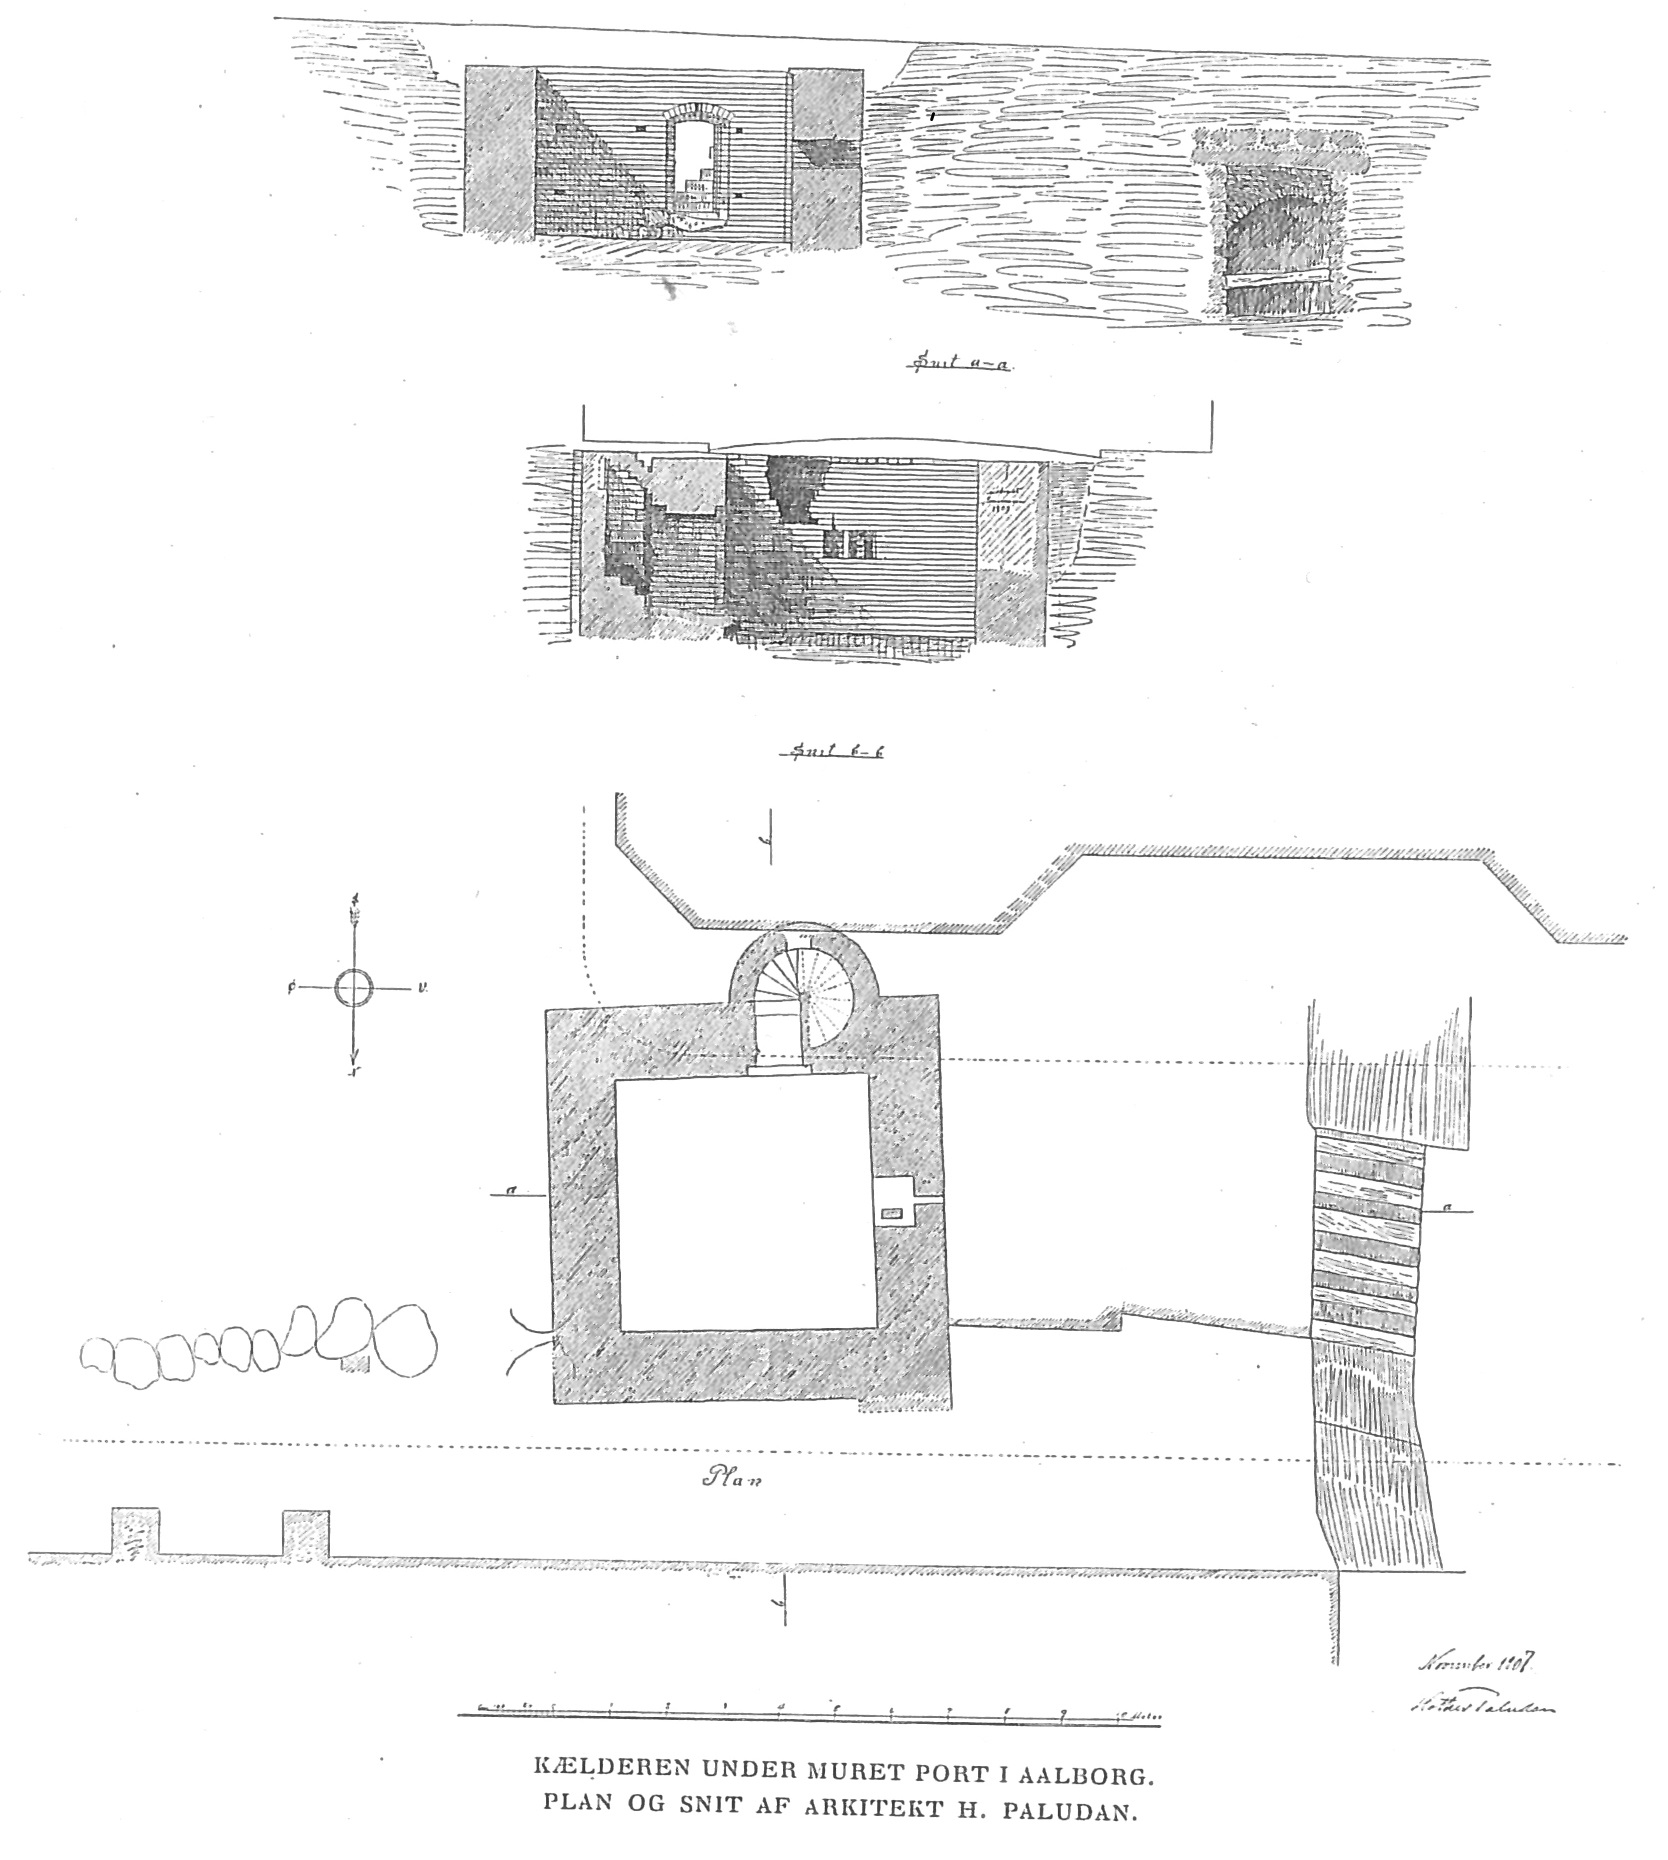
\includegraphics[width=\textwidth]{figures/sketch0.jpg}
	\caption{The dungeon beneath Vesterport in Aalborg, plan and section by architect H. Paludan \cite{Jensen1909}}\label{fig:sketch0}
\end{figure}

\begin{figure}
    \centering
        \begin{subfigure}[h!]{0.7\textwidth}
    	\centering
        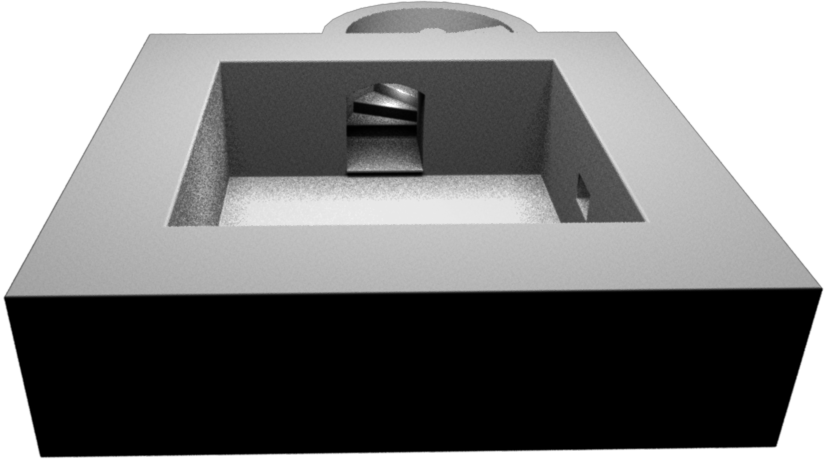
\includegraphics[width=\textwidth]{figures/model.png}
        \caption{The model of the dungeon, untextured}\label{fig:model}
    \end{subfigure}
    \begin{subfigure}[h!]{0.7\textwidth}
    	\centering
        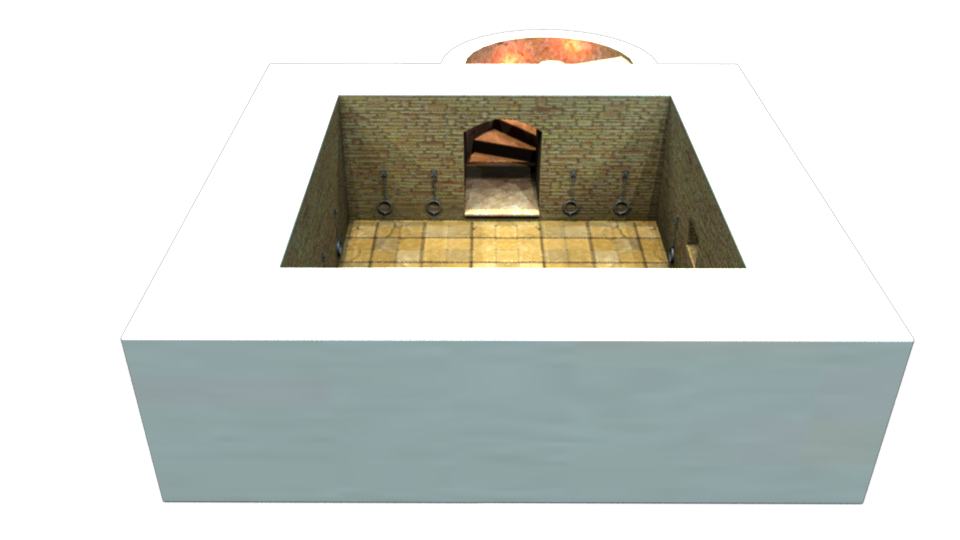
\includegraphics[width=\textwidth]{figures/model_total.png}
        \caption{The full model, with textures}\label{fig:total}
    \end{subfigure}
    \begin{subfigure}[h!]{0.7\textwidth}
    	\centering
        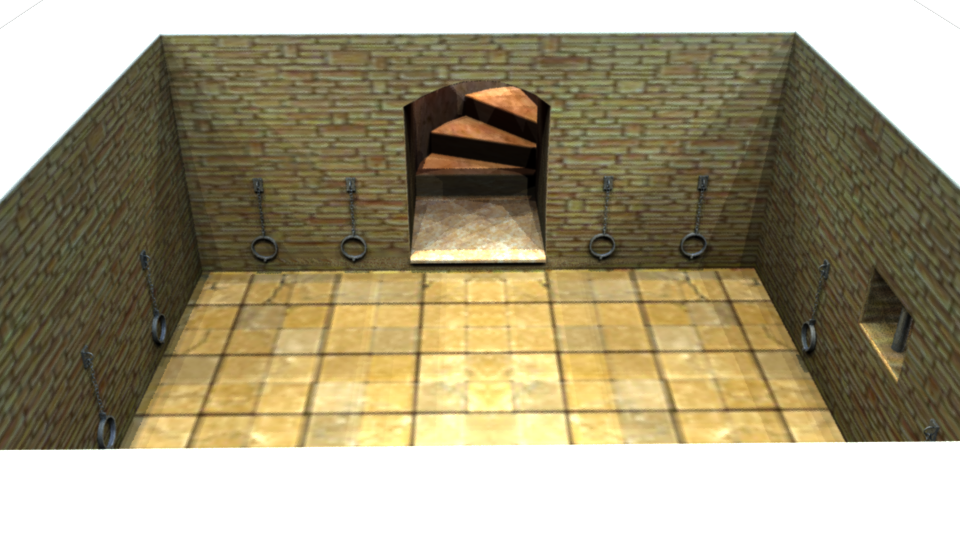
\includegraphics[width=\textwidth]{figures/model_long.png}
        \caption{The model as it will approximately look in the app}\label{fig:long}
    \end{subfigure}
    \caption{The model of \textit{Rakkerens Hule} to be used in the application}
\end{figure}

The base shape of the 3D model made from the sketches can be seen in Figure \ref{fig:model}. It is made of the geometric primitives: cube, cylinder, and pipe. The cube is used for the floor from which the walls and the staircase have been extruded, whereas the holes for the doorway and embrasure result from bridging the edges, left after the removal of strategic wall faces. A cylinder is used to make the bar in the prison window and the spindle directing the winding staircase. Lastly, half a pipe has been used to make the walls surrounding the staircase.%\pagebreak

Aside from the descriptions and sketches of the prison’s structure another source was found Jørgensen \cite{Jorgensen1934} and Jensen \cite{Jensen1909} which provided the description of the building materials for the prison. For instance they describe how the prison walls were constructed out of yellow bricks, the floor in the doorway consisted of granite, and the outside walls were covered with a layer of lime mixture. Images of the model with its textures can be seen in Figure \ref{fig:total} and \ref{fig:long}.

\begin{wrapfigure}{l}{0.2\textwidth}
   \centering
   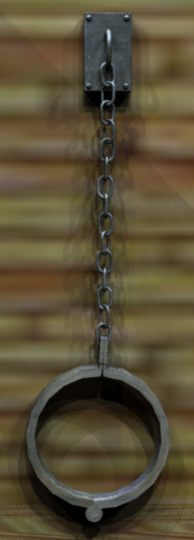
\includegraphics[width=0.18\textwidth]{figures/chainmodel.png}
   \caption{Close-up of a chain from the dungeon model}\label{fig:chain_model}
\end{wrapfigure}

Like the prison itself, the models of the chains is based on the design of real chains from the renaissance period found during archeological excavations, sketched by Carl Wognsen \cite{Riismoller1961}, see Figure \ref{fig:chains}. Primarily the illustration of the neck iron (Figure \ref{fig:chains1}) has been used since only the neck iron is meant to be attached to a wall in the dungeon. However, the chain part of the handcuffs has inspired the design of the chain device connecting the neck iron to the prison wall.

\begin{figure}
    \centering
    \begin{subfigure}[h!]{0.3\textwidth}
        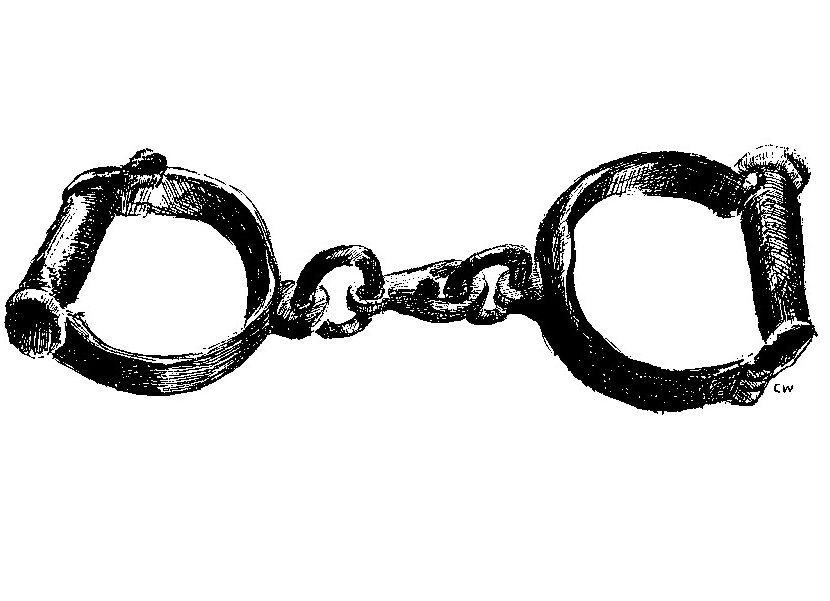
\includegraphics[width=\textwidth]{figures/chains0.jpg}
        \caption{Full illustration of handcuffs}\label{fig:chains0}
    \end{subfigure}
    \hfill
    \begin{subfigure}[h!]{0.3\textwidth}
        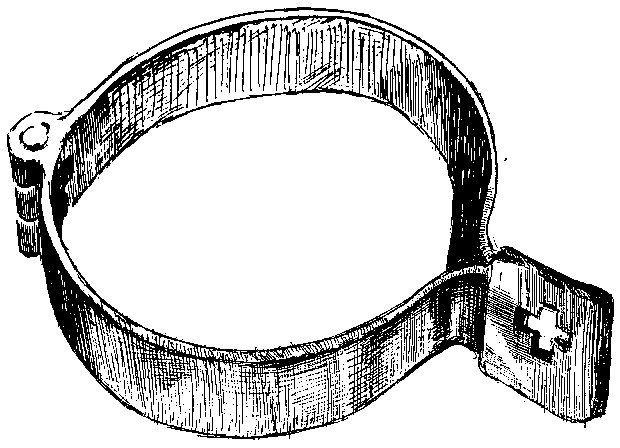
\includegraphics[width=\textwidth]{figures/chains1.jpg}
        \caption{Neck iron from the renaissance period. The cross shaped hole is for the chain}\label{fig:chains1}
    \end{subfigure}
    \hfill
    \begin{subfigure}[h!]{0.3\textwidth}
        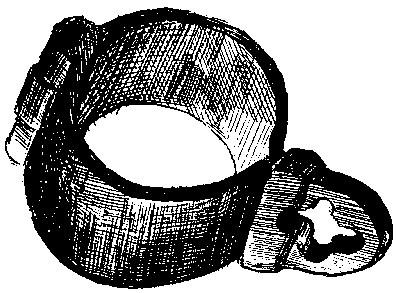
\includegraphics[width=\textwidth]{figures/chains2.jpg}
        \caption{Foot shackle from the renaissance period}\label{fig:chains2}
    \end{subfigure}
    \caption{Handcuffs from the town hall basement. Similar handcuffs may have been used in the dungeon. Illustration by Carlo Wognsen \cite{Riismoller1961}}\label{fig:chains}
\end{figure}

The 3D model is constructed from the primitives: pipe, cube, sphere, cylinder, and torus, textured with an iron texture, and it can be seen in its finalised version in  Figure \ref{fig:chain_model}. 
Two pipes and a cylinder make up the neck iron. Here one large pipe added some extrusions and bridges forms the main part. Meanwhile, does the other smaller pipe together with the cylinder compose the hinge (located at the bottom in the figure). Last but not least is the wall attachment made of a cube, four spheres cut in half as the screws and a round torus from which toruses prolonged into a chain joint shape is put in series in order to become the chain that connects the wall attachment with the neck iron.

\subsection{Light Sources}
The light setting consist of directional lights, three point lights, a spotlight, and an area light. To have the model’s entirety lit up as if situated outdoor on an average Danish spring day \cite{DMI}, a directional light with a faint tone of warm yellow has been utilised to emit the sunlight. More directional light sources with pale bluish tones have further been added to imitate the scattering of sunlight by atmospheric molecules in the sky --- a phenomenon also called Rayleigh scattering or critical opalescence \cite{DOE} \cite{Renn2005}. For the lighting of the staircase section a spotlight is used. Additionally, the staircase is lit up by three point lights with a deep orange tone to emulate torches hanging on the curved wall which can be seen in Figure \ref{fig:interior0}. Finally, an area light has been used to cast the light deriving from the embrasure hole, see Figure \ref{fig:interior1}.

\begin{figure}[h!]
    \centering
    \begin{subfigure}[h!]{0.8\textwidth}
    	\centering
        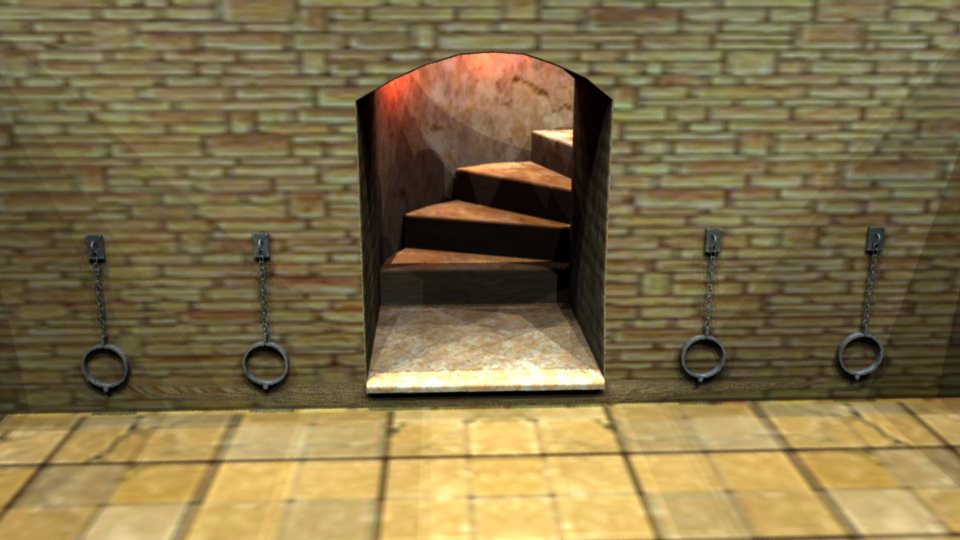
\includegraphics[width=\textwidth]{figures/interior0.png}
        \caption{The door in the dungeon, with visible staircase}\label{fig:interior0}
    \end{subfigure}
    \begin{subfigure}[h!]{0.8\textwidth}
    	\centering
        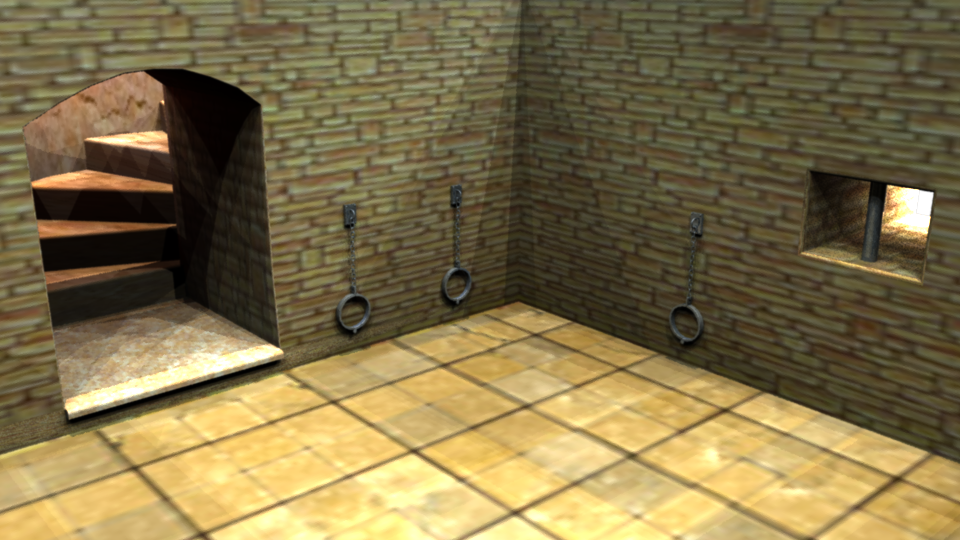
\includegraphics[width=\textwidth]{figures/interior1.png}
        \caption{The door, chains and window in the dungeon}\label{fig:interior1}
    \end{subfigure}
    \caption{Close-up of the interior of the model}\label{interior}
\end{figure}

\chapter{Evaluation}\label{ch:evaluation}
\section{Objective and Method} 
Set in relation to the problem formulation, the purpose of this evaluation is to see if using AR during a guided tour will have either a significant positively or negatively effect on the user experience when compared to a regular guided tour without the usage of AR. This is done in order to test whether incorporating AR will be beneficial during guided tours or not. 

To test this two similar versions of a guided tour has been arranged in cooperation with a tour guide from Aalborg Guideforening connected to the project through VisitAalborg - one with AR and one without AR. For the test to not suffer from fatigue by a repetitive experience within the participants testing the two tour versions, the research method between-subjects (often used within the scientific discipline of psychology when comparing two conditions [Citation] \todo{cite{Charness et al. 2011})} is chosen to be used. This method is used together with the quantitative methodology \textit{survey research} - used as the primary source for data collection.

The data collected from the conducted experiment by Likert scales is considered ordinal measurements. To analyze ordinal responses a nonparametric test is recommended to be used. Moreover the design of the experiment is unpaired, meaning each participant only tests one of the two tour versions. Because of this the nonparametric Wilcoxon Rank Sum Test should be used for the analysis. For the calculations of the data the significance level has been set to 0.05.

\todo{Missing: Approach inspired by add sources, References to similar studies and their test methods, Experience aspects/parameter}

\section{Setting}
The test will consist of a guided tour of app. 30 minutes, with two groups of participants. It will take place in Aalborg city centre during the morning. The guide will be Inge Vestergaard from Aalborg Guideforening. The guided tour will start at Gammeltorv then continue onto the area where Rakkerens Hule is located. Here one group will experience the AR application. The tour will finish off with the old monastery Helligåndsklosteret before returning to Gammeltorv. 

During the test two group members will follow the tour with video cameras and the necessary marker for the AR application. The other two group members will stay at Gammeltorv to prepare the second group and to be ready to hand out the end of test questionnaires to the first group. 

This makes the required items needed for this test:
\begin{itemize}
\item A video camera
\item A marker for the AR application
\item The questionnaires
\item Consent forms
\item The participants' android phones
\item Clipboards for the questionnaires
\end{itemize}



\section{Procedure}
\todo{Describe how we got the participants}
For the test a timeline was created, since it was only being conducted once and it required coordinating with both the guide, the project group and the participants. Beforehand the participants were split into two groups so as the second group would not have to wait for the first group to finish. 

\begin{tabular}{l p{12cm}}
09:00 & - The project group meets up at Gammeltorv to prepare \\
09:45 & - Evaluation team 0 meet up at Gammeltorv \\
 & - Consent forms are presented and the procedure is explained \\
10:00 &   - Evaluation Team 0 starts the guided tour \\
10:10 & - Evaluation Team 1 meets up at Gammeltorv \\
 & - Consent forms are presented and the procedure is explained including the AR application \\
10:30 & - Evaluation Team 0 finishes the guided tour and are handed the questionnaires \\
 & - Evaluation Team 1 starts the guided tour
\\ 
11:00 & - Evaluation Team 1 finishes the guided tour and are handed the questionnaires \\
11:xx & - When Evaluation Team 1 is finished the test ends \\
\end{tabular}


\section{Statistical analysis of results} 
\subsection{hypothesis}
Hypothesis based on research question 2:

In what way does the addition of an AR application affect tour goers’ curiosity to learn more, if at all?

\begin{itemize}
\item H1(0) - After experiencing a tour with the AR application, participants report the same level of curiosity as that of the participants who experienced the tour without the AR application. 
\item HA - After experiencing a tour with the AR application, participants report a different level of curiosity than that of the participants who experienced the tour without the AR application. 
\begin{itemize}
\item H1a: After experiencing a tour with the AR application, participants report a higher level of curiosity than that of the participants who experienced the tour without the AR application.
\end{itemize}
\end{itemize}

Hypothesis based on research question 3:

In what way does the addition of an AR application affect whether tour goers find the tour entertaining, if at all?

\begin{itemize}
\item H2 - After experiencing a tour with the AR application, participants agree with the statement that they were entertained to the same degree as that reported by the participants who experienced the tour without the AR application. 
\item HA - After experiencing a tour with the AR application, participants agree with the statement that they were entertained to a different degree than that reported by the participants who experienced the tour without the AR application. 
\begin{itemize}
\item H2a: After experiencing a tour with the AR application, participants agree with the statement that they were entertained to a higher degree than that reported by the participants who experiences the tour without the AR application. 
\end{itemize}
\end{itemize}

Hypothesis based on research question 4:

In what way does the addition of an AR application affect whether tour goers are distracted during the tour?

\begin{itemize}
\item H3 - After experiencing a tour with the AR application, participants report the same level of distraction as that of the participants who experienced the tour without the AR application. 
\item HA - After experiencing a tour with the AR application, participants report a different level of distraction than that of the participants who experienced the tour without the AR application.
\begin{itemize}
\item H3a: After experiencing a tour with the AR application, participants report a higher level of distraction than that of the participants who experienced the tour without the AR application.
\end{itemize}
\end{itemize}
\chapter{Discussion}\label{ch:discussion}
Throughout the project, there were some aspects that could have been done in a different manner, and, in that way, the overall quality of the project could have been improved. In this chapter, those aspects are described in detail.

\section{Quality of results}
The data samples collected from the test have been very small. Therefore, making general conclusions based on standalone data would be considered very unreliable in this case. For instance, there were 11 and 13 participants in the control group and test group respectively. Meanwhile, there were seven rating options on the rating scale for the participants to select from in the questionnaire. Therefore, if the participants differed much in their opinion about the experience, the result could easily be so spread out that the data collected would be meaningless. In relation to this concern is another factor that may have reduced the reliability of the test which is the limitation of time for the test (one hour), since this put a restriction to how many groups could experience the tour. Because that, for each of the two conditions there would be only one group testing which have made it impossible to seek for patterns to generalise from e.g. by averaging numbers.

In the questionnaire there may be some disruptive data connected to the SAM based question concerning the participants’ arousal, cf. Appendix \ref{app:questionnaire}. This was due to poor understanding of the word among the participants in this particular context, which can have had an impact on the reliability of this specific result.

Concerning the results received from the video analyses the video data collected has been inflicted by a series of external disruptions like loud noise and high traffic with moving vehicles --- known conditions, though beyond the group’s control. However, this could not be avoided due to the changing nature of a tour site. Doing the test at a quieter place of course would be a possibility, but then the test would suffer in the feel of actual being on the site watching what lies underground. Therefore, although the number of distractions among the participants observed in the videos may have increased due to the noise and traffic in the background, it is considered to be the most realistic scenario and therefore desirable. Furthermore, these conditions may also have influenced the answers given in the questionnaire. Especially in regards to answers given to the questions 13 and 14 asking into the participants’ experience of distraction at the site, cf. Appendix \ref{app:questionnaire}.
Both for the video data and the questionnaire answers it is therefore reasonable to consider parts of the data to be unreliable. 

To heighten the validity of the results, different forms of data collection methods (questionnaire, video recording, and interview) have been used to gather both quantitative and qualitative data, which help balance each other out if used in combination . Furthermore, this has been done to enable the usage of methodological triangulation also referred to as mixed method research \cite{Kennedy}. Using triangulation can validate the results by cross verification as it investigates whether or not the varying forms of data confirm each other, and thereby reaches to the same conclusion. Moreover, the triangulation of data helps to rectify bias. This could, for instance, be procedural bias such as participants who rush their answers in order to quickly finish of the questionnaire, or measurement bias like response bias, which can be counteracted by combining self-reported and observational research \cite{Kennedy}. Although the latter could have been improved by using investigative triangulation for the analysis of the videos, since two researchers are likely to have different perspectives. Therefore a utilisation of two or more observers that counterbalance one another would improve the validity of the results when compared to only having one investigator perform the analysis \cite{Kennedy}. The lack of data logged from the application is a deficiency in the gathered data. This could have illustrated how participants used the application e.g. activation time and orientation, which could have added to the quantitative data collection. The reason for leaving out data logging was due to the Danish legislation about privacy policy concerned with using data collected from people’s phones cf. The Danish Data Protection Agency \cite{Datatilsynet}.

A factor to consider in the execution of the test that might have affected the validity is the participants’ backgrounds. Although the guide explained that the people going on tours come from a variety of backgrounds such as families with parents and children, elderly people, bachelor parties, etc., cf. Appendix \ref{app:guide_emails}, the participants used for the test consisted only of people within the age range 20 to 31 and were recruited primarily among students. This has resulted in the sample having an omission bias, for which reason it cannot be said to be truly representative of the users typically using the guided tours. This could easily have been managed differently by a change in the procedure for recruiting participants. This was done by posting an event on Facebook. It was shared only within the medialogy group and among the group members’ friends and families together with recruiting locally by asking medialogy students at campus.

Another factor which could influence the validity of the test is the recruited participants’ self-interest, both in regard to their personal interest to the content of the tour as well as their interest in the AR technology. As mentioned above, many of the recruited participants were medialogy students who presumably have a technical background with an interest in new technologies. This could potentially make them biased towards a higher ranking of the tour version with AR incorporated. Although the questionnaire results imply this to not be the case, this could be due to the procedure not having each of the two groups try out both versions. For this reason, the participants’ were not able to compare the two versions. Choosing this procedure therefore may have increased the validity in regards to this aspect.  

\section{Future work},
There are also several aspects of the project that could be interesting to look into as part of future research. 

One of them is to test a VR version of the design in order to acquire the knowledge about how VR would influence the guided tour experience compared to AR. This might be interesting to compare based on it being a lot easier to leave out the AR aspect of an app and just have an entirely digitally rendered version of the app. This would allow tour goers to also look at the model later without being in the correct spot. However, it might lessen the immersion of the tour that the thing being shown on screen has no direct link to the surroundings. This makes it an interesting angle to research, since it would be simpler to make, but might lose some immersion compared to AR. 

Another aspect that would be curious to investigate is a markerless AR implementation of the product. This would allow for an easier use of the final product since there would not be a necessity to carry around a rather large marker during the guided tour.
  
Another possible point of interest arises due to how the human cognition works. To be more exact, humans process auditory and visual information through different channels, and, unfortunately, there is a possibility to overload those channels. In order to increase the effectiveness of acquiring new information, an individual should be able to mentally connect the visual and auditory information and organise it in a coherent manner \cite{audiovisual_learning}. Therefore, it would be interesting to see how to make the final product in such a way that the aforementioned possible complications could be avoided and the overall user experience could be improved.

Implementing realistic lighting could also be a part of future work, since that could make the 3D model look more natural in the outdoor setting. In that way, the 3D model would seem more like a part of the urban environment, and less like a foreign element. Thus, the overall user experience could be improved.

Furthermore, another possibility to improve the design could be to integrate actual pictures of the site into an AR system, as suggested by Inge Vestergaard, who is the guide that aided with the evaluation testing. Besides that, integrating the AR on other sites of the tour might be a good idea, since it would give a better understanding to the users of how certain urban elements might have looked in the past, and give results that are more influenced by the application so they will be more clearly comparable. 

The main reason why the aforementioned aspects are not part of the current report is lack of time due to organisational issues. They were mainly caused by having some trouble with establishing a collaboration with a third party. At first, there was made considerable effort to work together with a museum. However, the museum association did not show interest in our project. After the official rejection, VisitAalborg was contacted, which then resulted in a collaboration. 


\chapter{Conclusion}\label{ch:conclusion}
Put a conclusion here \todo{remember conclusion}
\printbibliography[heading=bibintoc]
\label{bib:mybiblio}
\appendix
\chapter{EDA and IBI graphs from preliminary test}\label{app:preliminary}
The following pages contain the graphs generated from the IBI and EDA results gathered from the preliminary test.
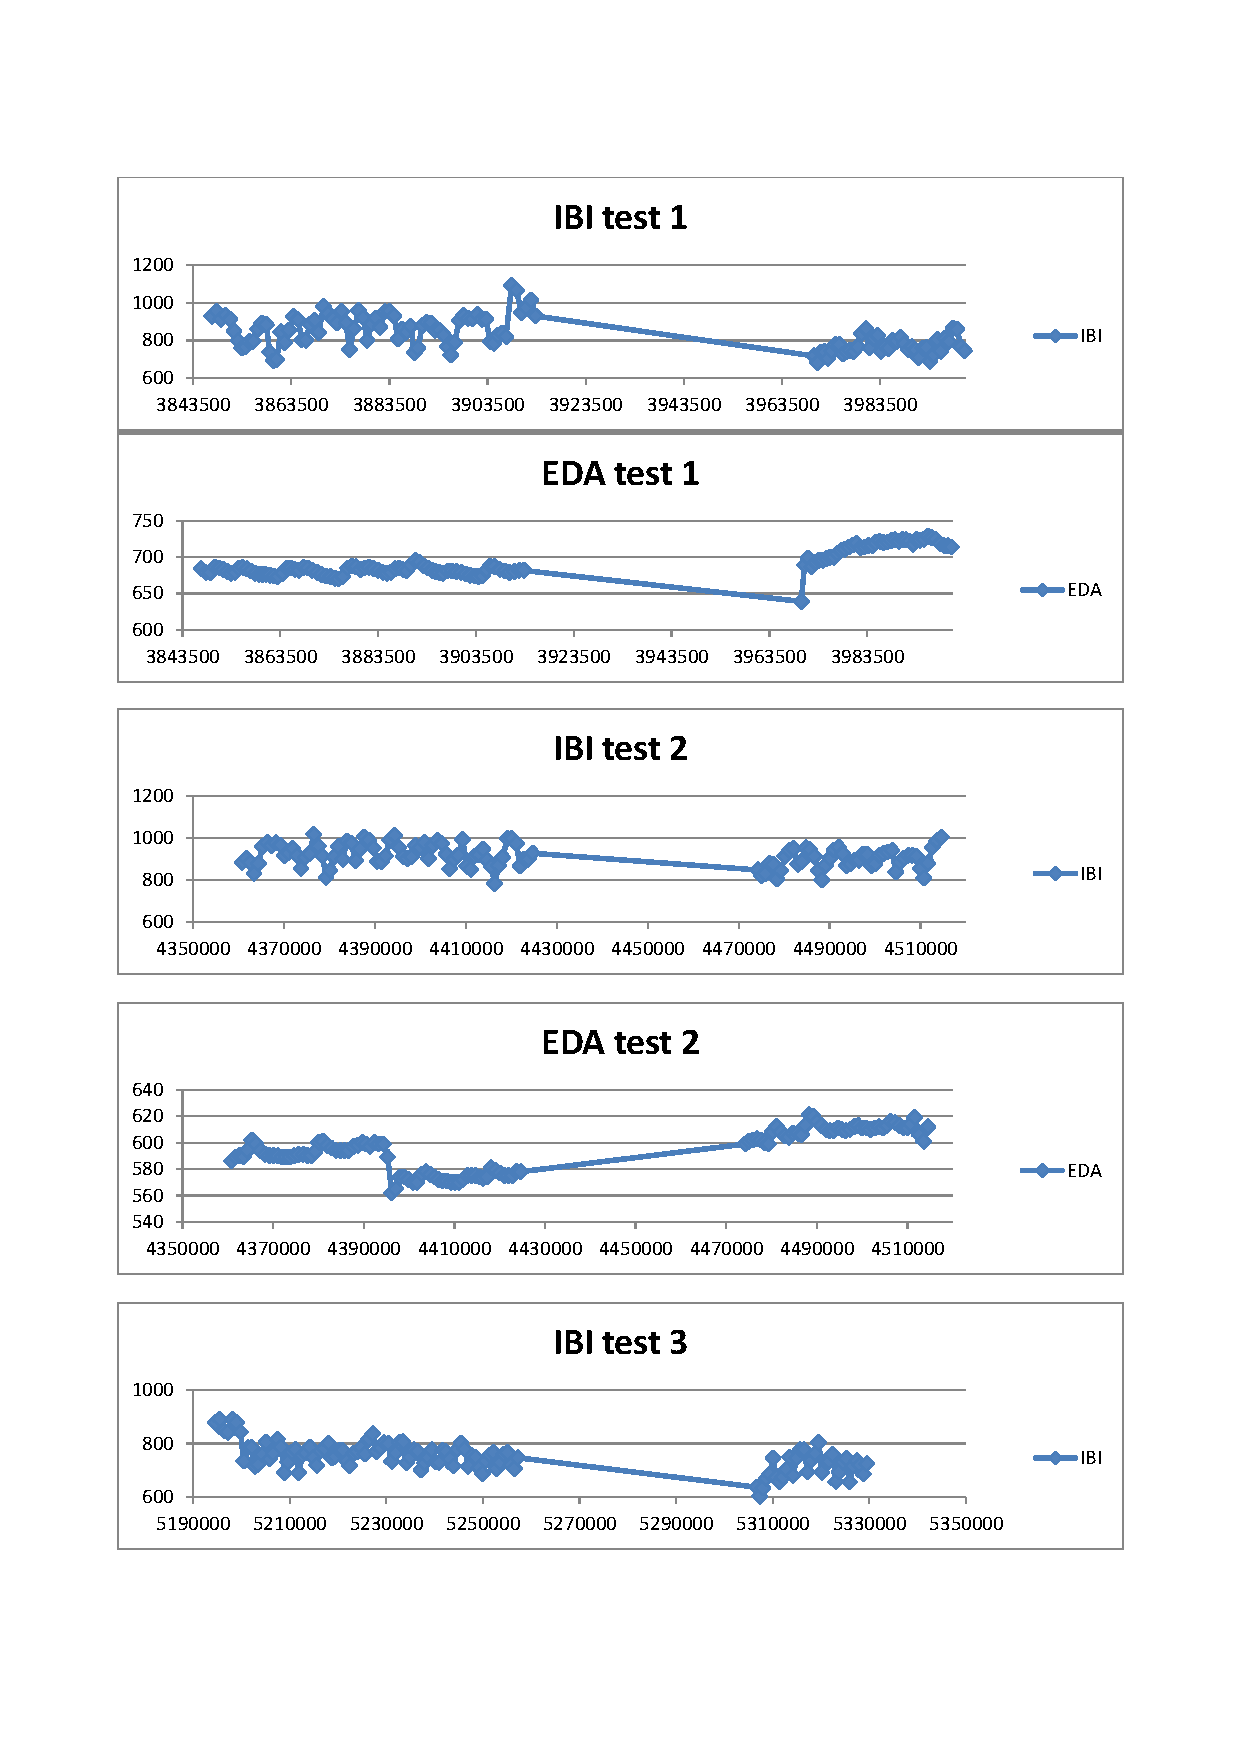
\includepdf[pages=1-4]{sections/graphs.pdf}

\chapter{Questionnaire}\label{app:questionnaire}
The following pages contain the questionnaire given to participants of the test. The first page contains sixteen statements. Participants mark to which degree they agree with these statements. The second page contains two SAM mannekin scales, on which participants may mark their level of pleasure and arousal, respectively. It also contains a field in which participants may add other comments.

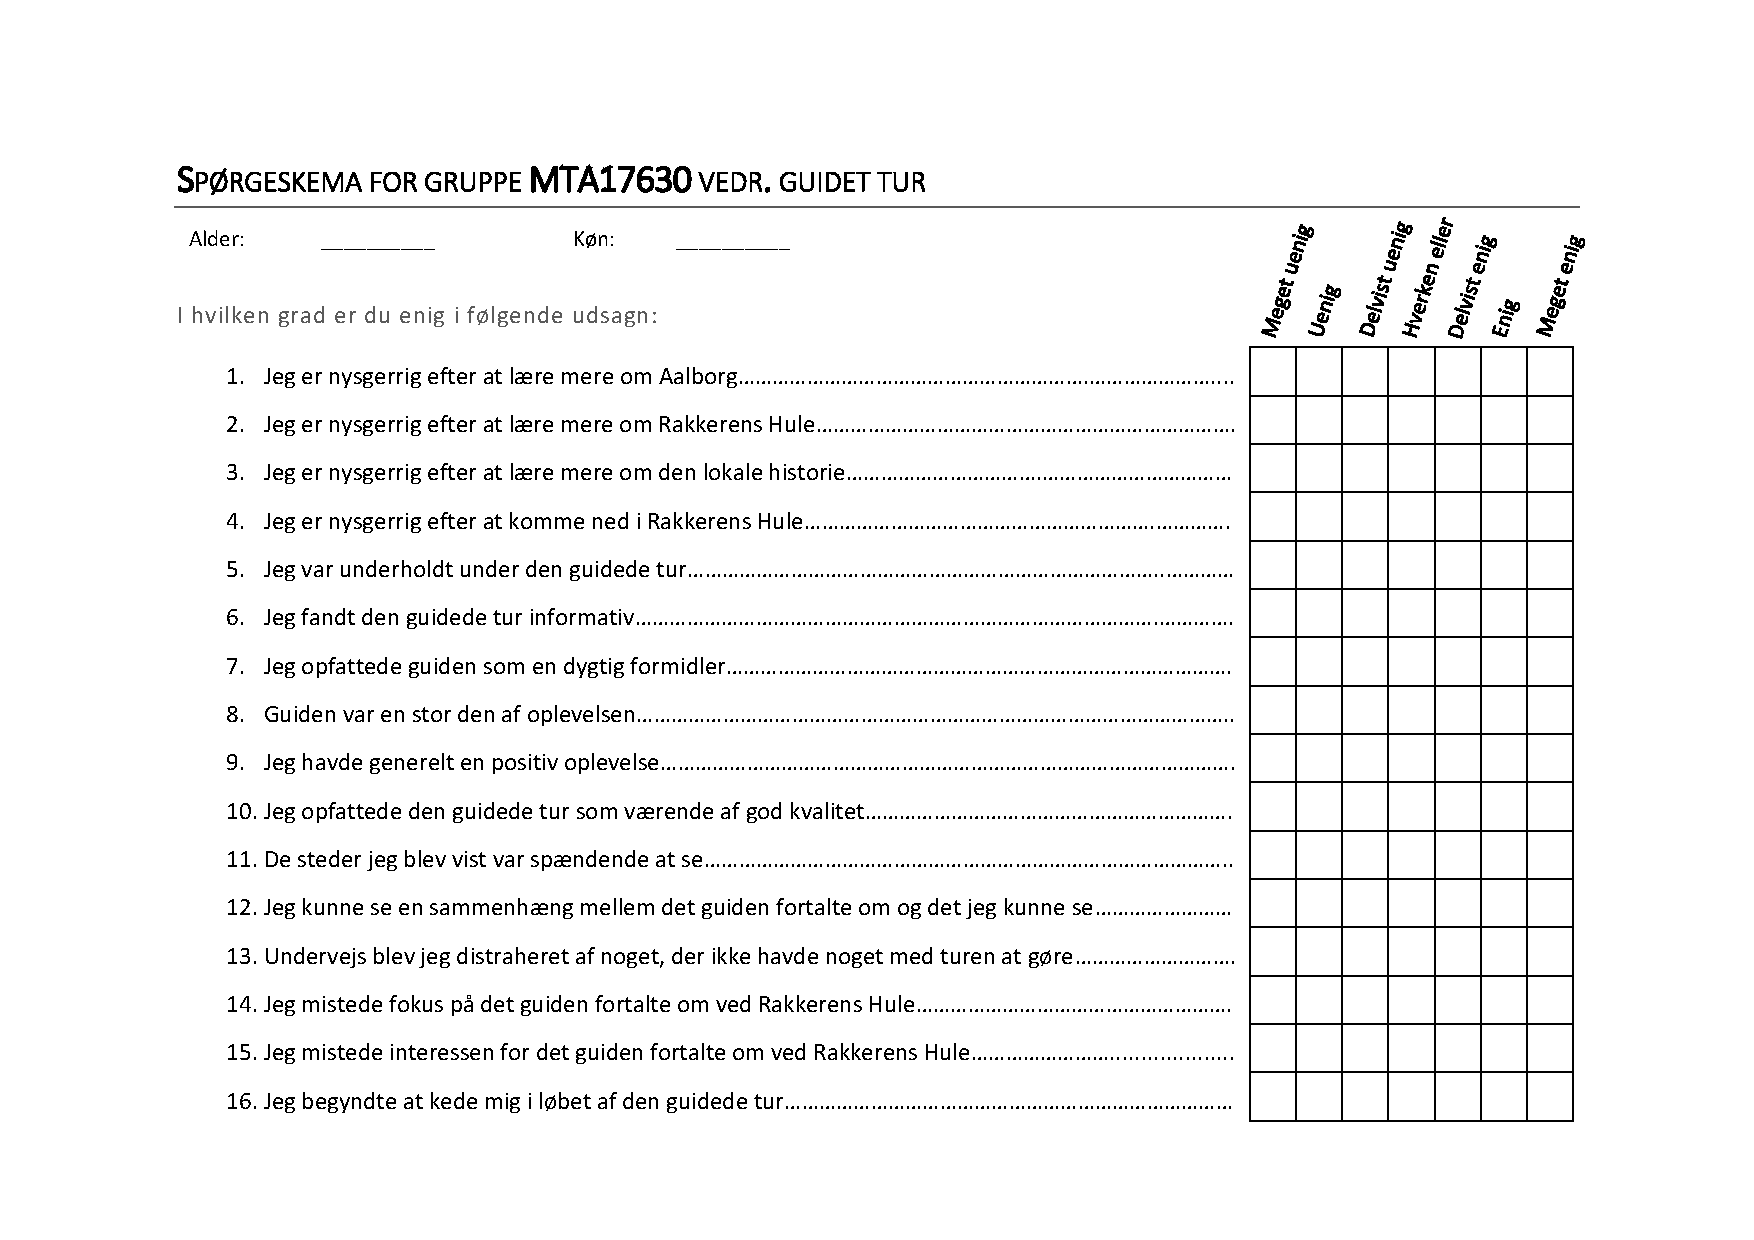
\includepdf[pages=1-2]{sections/questionnaire.pdf}


\chapter{Results from the questionnaire}\label{app:questionnaire_results}
The following pages contain responses from the questionnaire rating scale statements, as well as the SAM mannekin questions. The rating scale statements are labeled \textit{Q1-Q16}, and the SAM questions are labeled \textit{SAM pleased} and \textit{SAM aroused}. The questions themselves can be seen in Appendix \ref{app:questionnaire}. Each participant's age and gender is given, as well as their response to each question. The numbers provided for the rating scale statements respond to the following responses:

\paragraph{-3:} Meget uenig (strongly disagree)
\paragraph{-2:} Uenig (disagree)
\paragraph{-1:} Delvist uenig (somewhat disagree)
\paragraph{0:} Hverken eller (neither agree nor disagree)
\paragraph{1:} Delvist enig (somewhat agree)
\paragraph{2:} Enig (agree)
\paragraph{3:} Meget enig (strongly agree)\\
\\
The SAM responses (seen in Appendix \ref{app:questionnaire}) are labeled 1 through 5, from left to right.

\begin{figure}[h!]
    \centering
    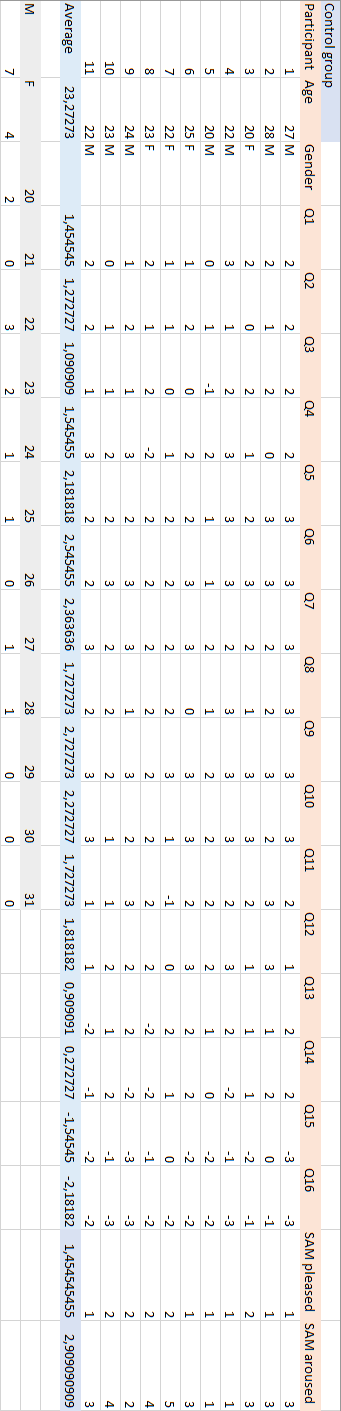
\includegraphics[scale=0.65]{figures/questionnaire_results_control.png}
    \caption{Responses to the questionnaire from the control group}\label{fig:responses_control}
\end{figure}

\begin{figure}[h!]
    \centering
    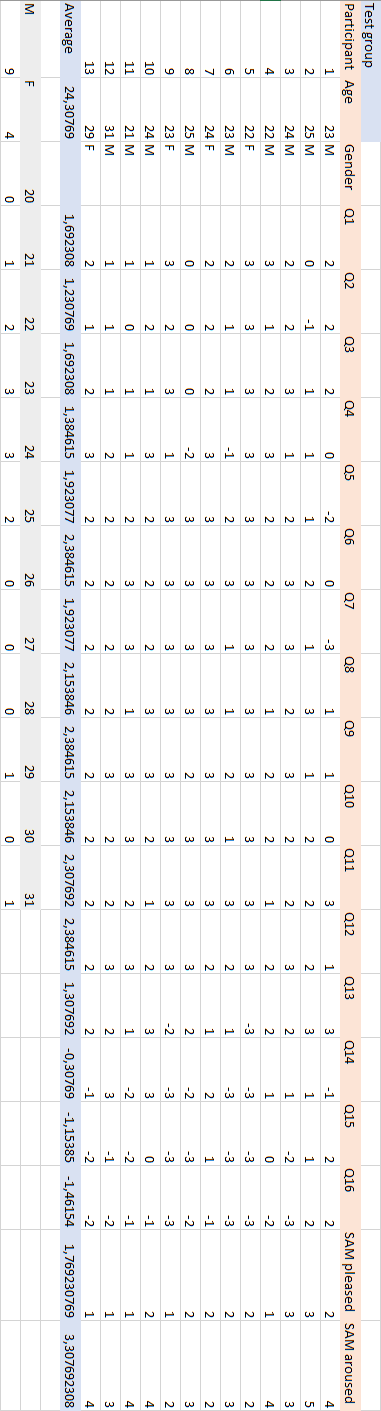
\includegraphics[scale=0.65]{figures/questionnaire_results_test.png}
    \caption{Responses to the questionnaire from the test group}\label{fig:responses_test}
\end{figure}
\chapter{Transcript of interview with the guide}\label{app:transcriptInterview}
Here is a transcript of the interview conducted with the guide Inge Vestergaard. The transcript is in Danish, as this was the language the interview was conducted in. 

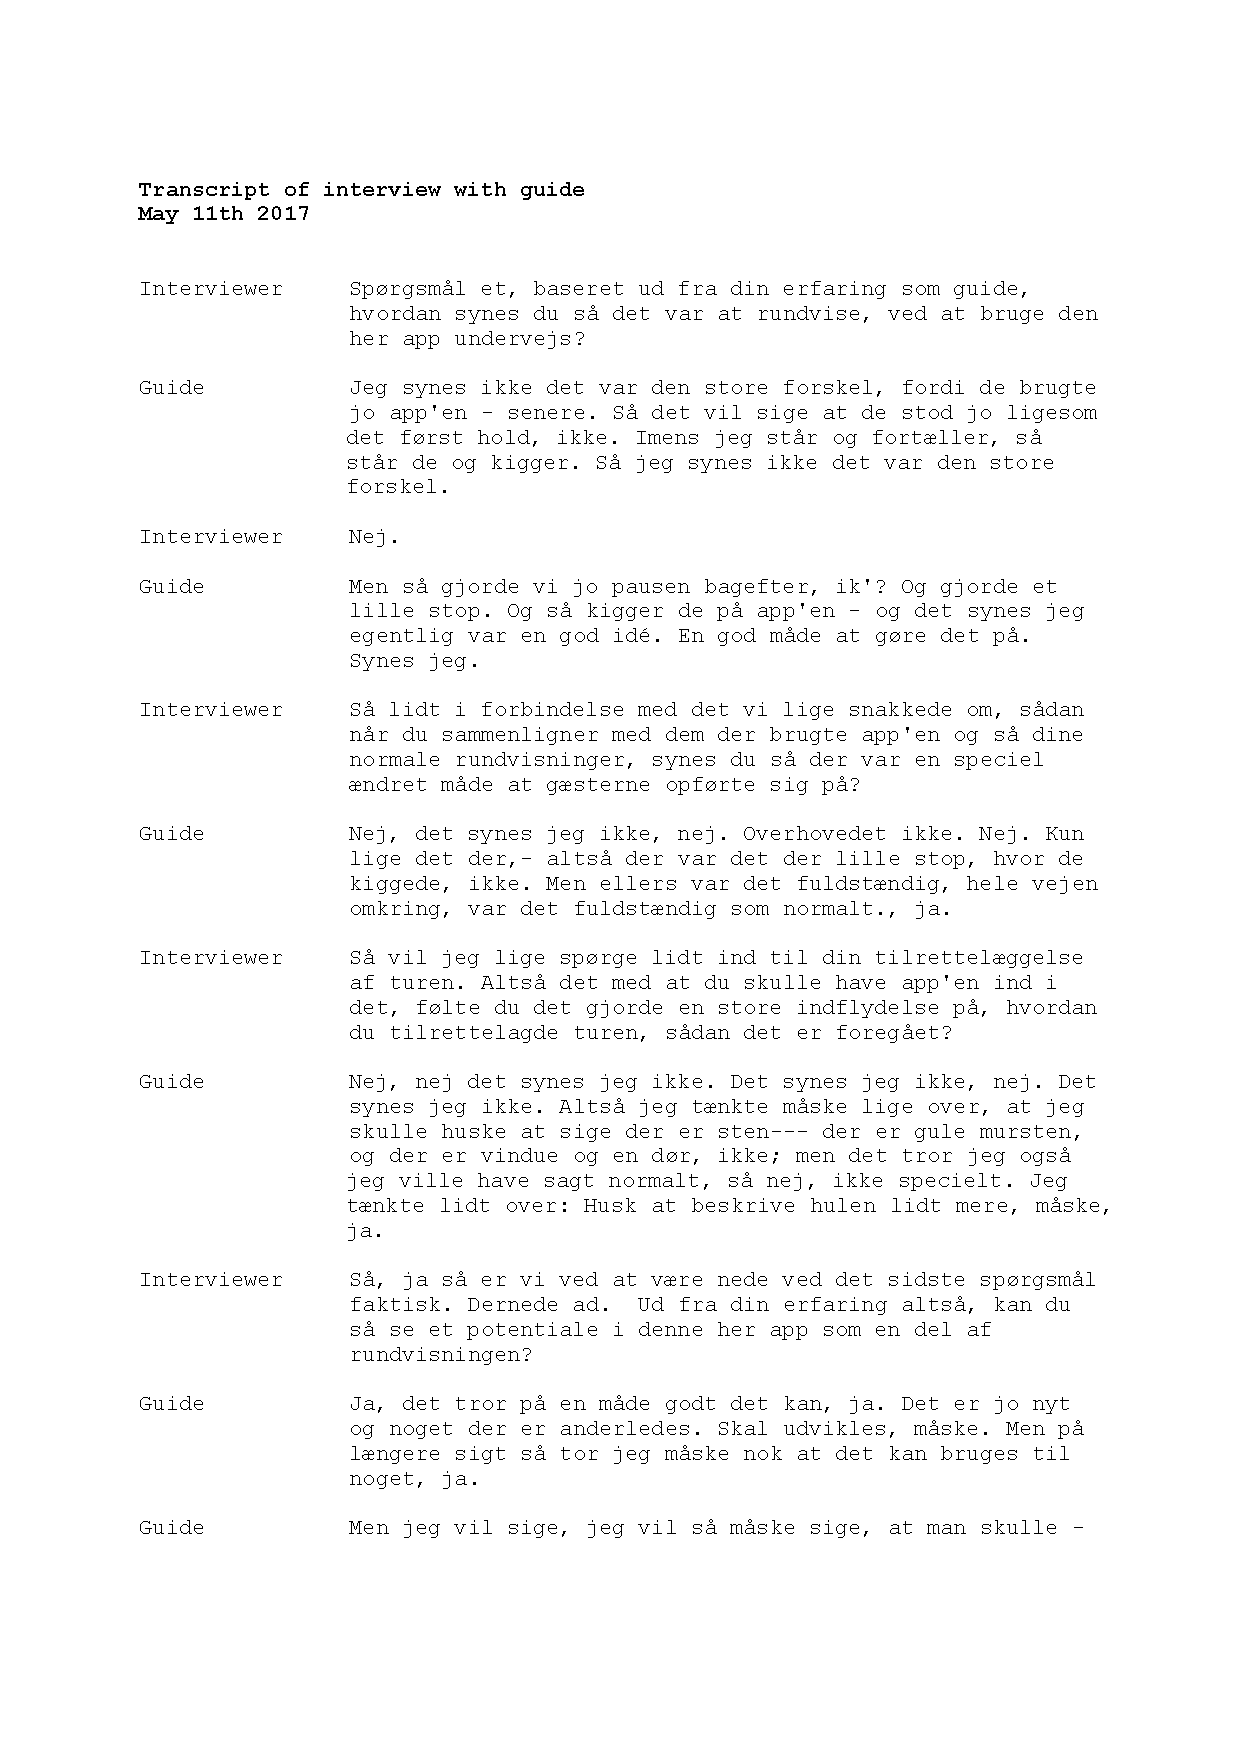
\includepdf{sections/transcriptInterview.pdf} 
\chapter{Video analysis of recordings of guide}\label{app:guide_results}
This is a log of the data analysis done in the program ELAN, of the video recordings of the guide at Rakkerens Hule.

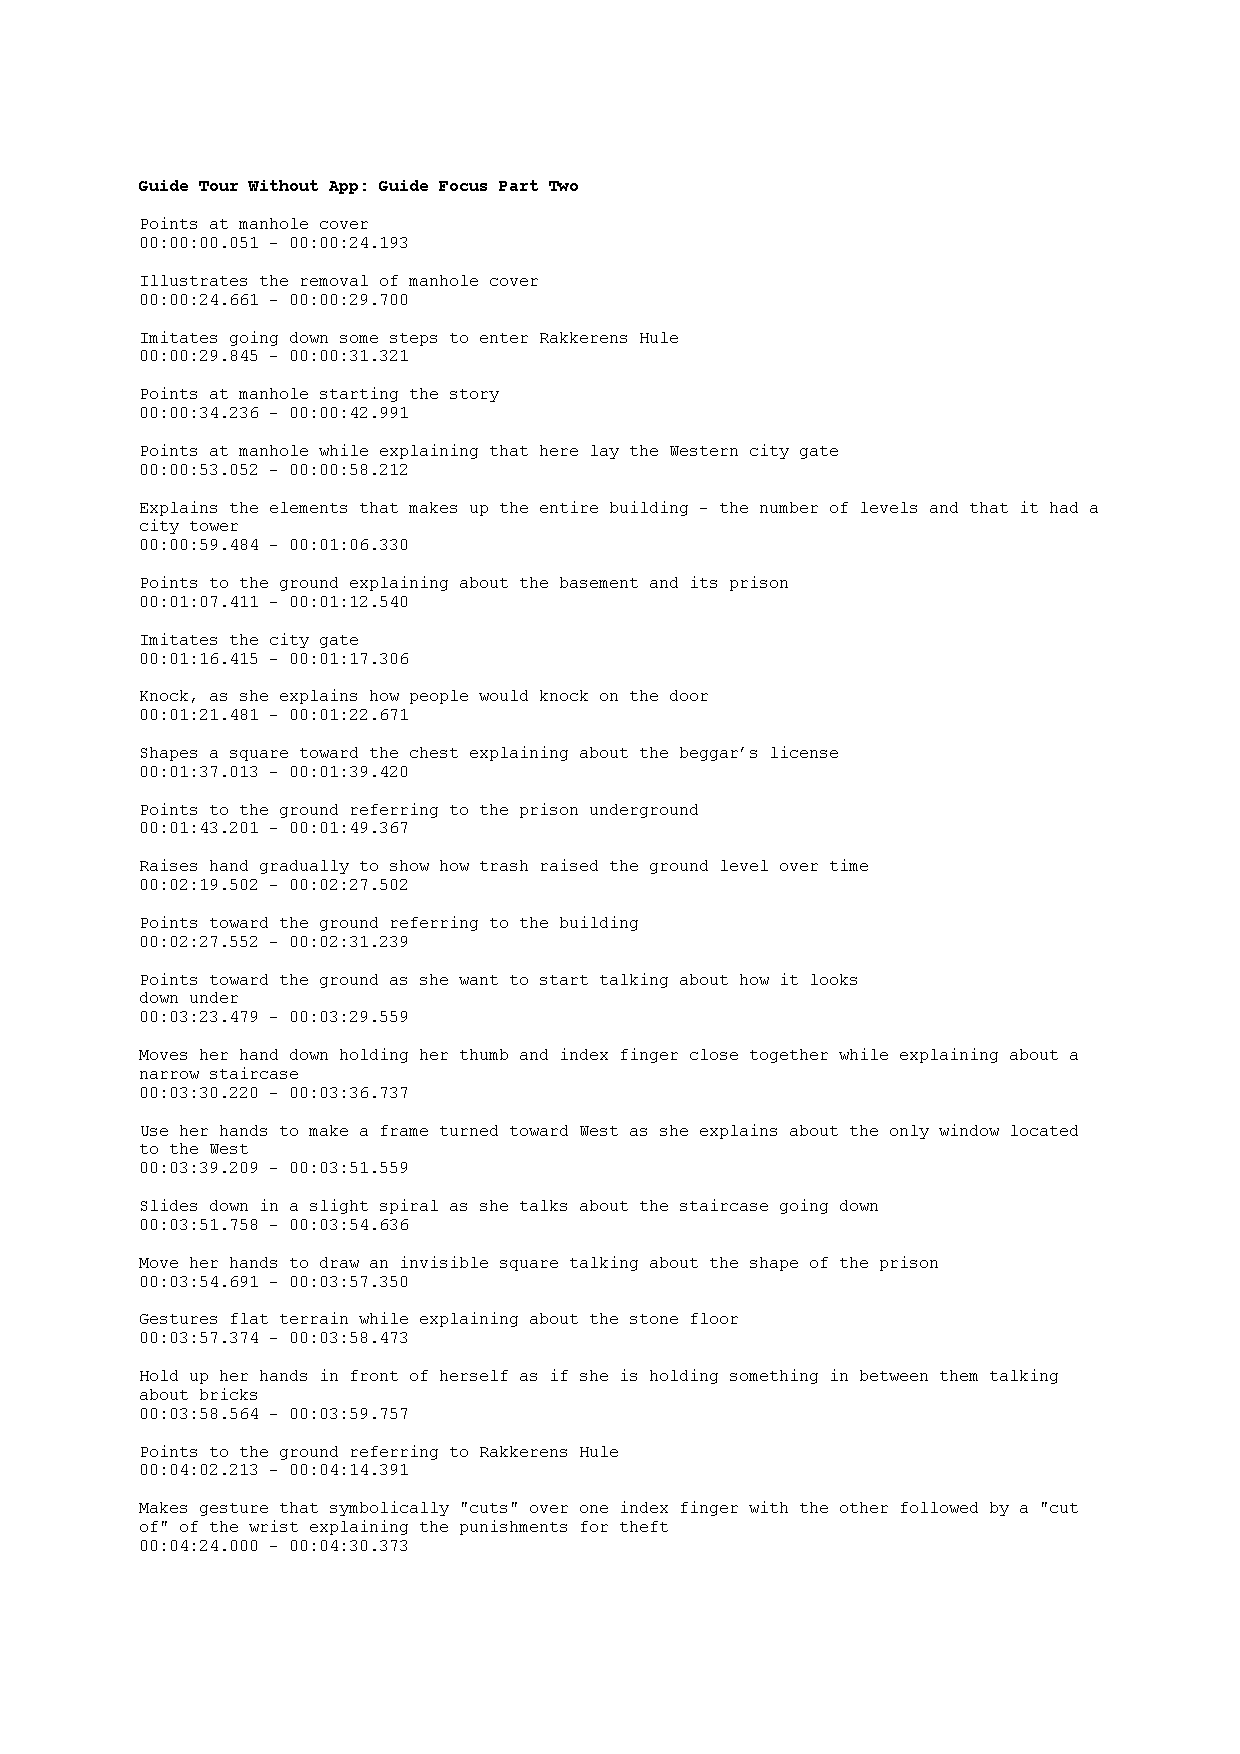
\includepdf{sections/guide_results.pdf}
\chapter{E-mail correspondence with collaborators}\label{app:guide_emails}
Here the e-mails exchanged between the group and the two collaboraters, VisitAalborg and Aalborg Guideforening can be found.

\includepdf{sections/inge_Emails.pdf}
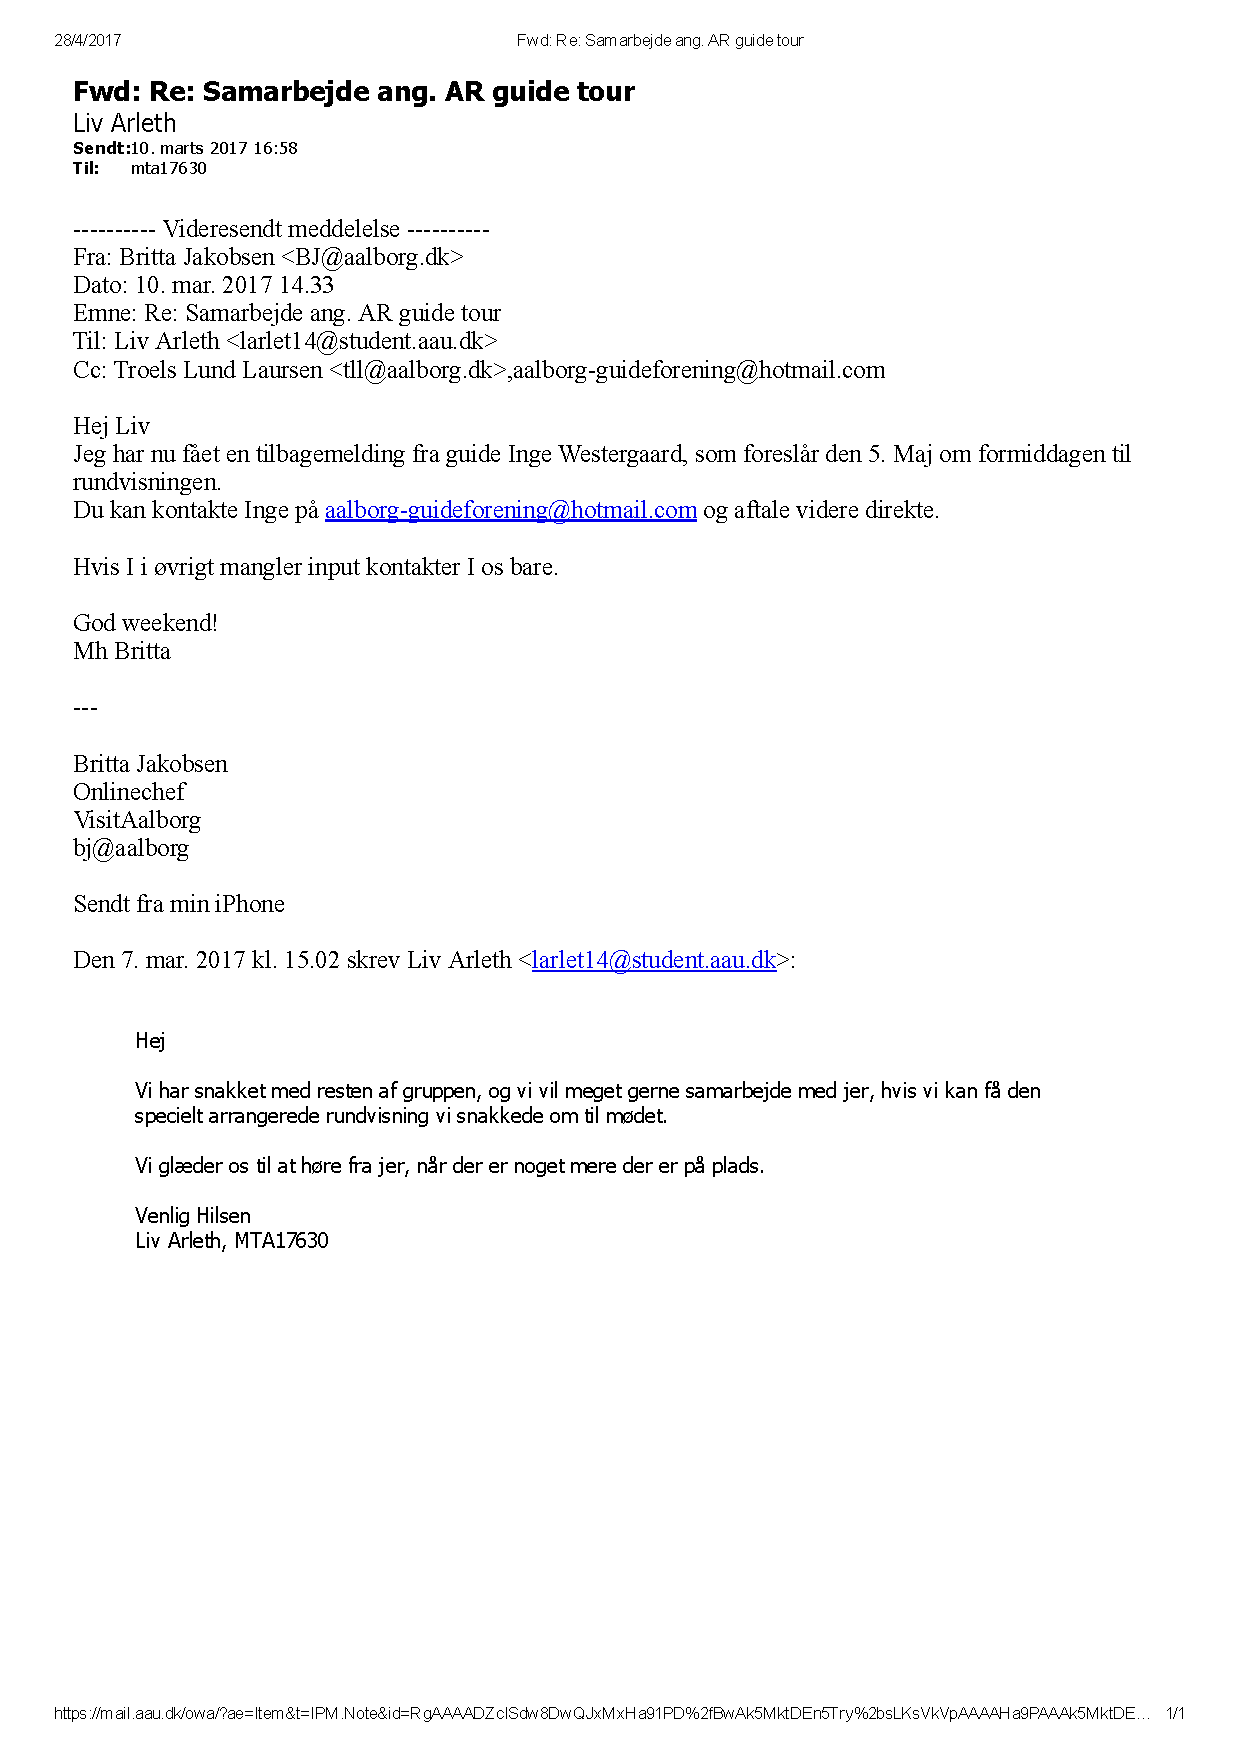
\includepdf{sections/VA_emails.pdf}


\end{document}
